\documentclass[xcolor={dvipsnames},10pt]{beamer}
%
% Choose how your presentation looks.
%
% For more themes, color themes and font themes, see:
% http://deic.uab.es/~iblanes/beamer_gallery/index_by_theme.html
%
\mode<presentation>
{
  \usetheme{Warsaw}      % or try Darmstadt, Madrid, Warsaw, ...
  \usecolortheme{default} % or try albatross, beaver, crane, ...
  \usefonttheme{default}  % or try serif, structurebold, ...
  \setbeamertemplate{navigation symbols}{}
  \setbeamertemplate{caption}[numbered]
}

\usepackage[english]{babel}
\usepackage[utf8]{inputenc}
\usepackage{animate}

\usepackage{hyperref} % pour insérer des liens

\usepackage{epstopdf} %converting to PDF
\usepackage[export]{adjustbox} %for large figures

\usepackage{graphicx} % for graphicspath
\graphicspath{{../images/}}

\usepackage{multicol}
\title[Le modèle de Hindmarsh-Rose]{Étude du premier modèle de Hindmarsh-Rose}

%\usepackage[dvipsnames]{xcolor}

\usepackage{hyperref} % pour insérer des liens

\usepackage{array}
\newcolumntype{L}[1]{>{\raggedright\let\newline\\\arraybackslash\hspace{0pt}}m{#1}}
\newcolumntype{C}[1]{>{\centering\let\newline\\\arraybackslash\hspace{0pt}}m{#1}}
\newcolumntype{R}[1]{>{\raggedleft\let\newline\\\arraybackslash\hspace{0pt}}m{#1}}



\setbeamertemplate{navigation symbols}{\insertframenumber/\inserttotalframenumber}

\author{Vincent Matthys, Maureen Muscat et Mariène Wan}

\institute{Master 1 BIM \\ Université Pierre et Marie Curie}
\date{17/05/2017}

\begin{document}

\begin{frame}
\titlepage
\end{frame}

% Uncomment these lines for an automatically generated outline.
%\begin{frame}{Outline}
%  \tableofcontents
%\end{frame}

\section*{Introduction}

\begin{frame}{Introduction}

\begin{itemize}
  \item Nous nous intéressons au modèle suivant :

\begin{equation}
\left\{
\begin{array}{l l}
v'(t)= \displaystyle{\frac{w - v^3 + 3v^2 +I_{ap}}{c}} = f(v,w) & \text{ avec } c\neq 0\\
w'(t) = 1 - 5 v^2 - w = g(v,w) & \\
\end{array}
\right.
\end{equation}

 \item $c$ et $I_{ap}$ sont des paramètres
 \item c'est un modèle d'activité neuronale, $v$ représente la tension de la membrane du neurone.

\end{itemize}
\end{frame}

\begin{frame}
\tableofcontents % [currentsection]
\end{frame}
% Commands to include a block
% \begin{block}{Examples}
% Some examples of commonly used commands and features are included, to help you get started.
% \end{block}

% Commands to include a figure:
%\begin{figure}
%\includegraphics[width=\textwidth]{your-figure's-file-name}
%\caption{\label{fig:your-figure}Caption goes here.}
%\end{figure}
\section{Pour \texorpdfstring{$C=2$}{Lg}}

\subsection{Recherche des points d'équilibre}
\subsubsection*{Les nullclines}
\begin{frame}{Recherche des nullclines}
\begin{equation*}
\left\{
\begin{array}{l l}
v'(t)= \displaystyle{\frac{w - v^3 + 3v^2 +I_{ap}}{c}} = f(v,w) & \text{ avec } c\neq 0\\
w'(t) = 1 - 5 v^2 - w = g(v,w) & \\
\end{array}
\right.
\end{equation*}

\begin{align*}
\text{Nullcline\,pour\,v : } v' &= 0  &\Leftrightarrow w &= v^3 - 3 v^2 - I_{ap}\\
\text{Nullcline\,pour\,w : } w' &= 0 &\Leftrightarrow w &= 1-5v^2
\end{align*}
La nullcline de $v$ est de forme \textbf{cubique}. \\
La nullcline de $w$ est une \textbf{parabole}.
\end{frame}


\begin{frame}{Évolution du nombre de points stationnaires \\ quand I augmente}
\begin{columns}
	\begin{column}{0.5\textwidth}
		 \animategraphics[autoplay, width=7cm]{10}{gif/}{000}{159}
	\end{column}
	\begin{column}{0.4\textwidth}  %%<--- here
		\begin{center}
		\begin{tabular}{l l}
			$I_{ap}< - 1$ &  1 \\
			$I_{ap}= - 1$ &  2 \\
			$I_{ap} \in ]-1, 5/27[$ &  3 \\
			$I_{ap}=5/27$  &  2 \\
			$I_{ap}> 5/27$ &  1 \\
		\end{tabular}
		\end{center}
	\end{column}
\end{columns}
\end{frame}

\subsubsection*{Diagramme de bifurcation}

\begin{frame}{Allure du diagramme de bifurcation}
Les points d'équilibres vérifient $w = v^3 - 3 v^2 - I_{ap}$ et $w = 1-5v^2$.


\begin{equation*}
v^3 + 2 v^2 -1 =I_{ap}
\end{equation*}
\begin{center}
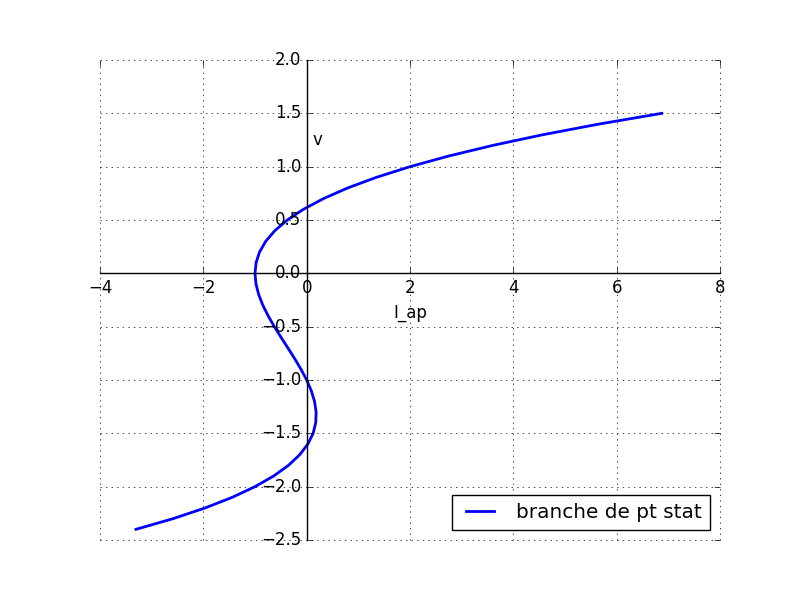
\includegraphics[width=0.6\textwidth]{bif1.png}
\end{center}
\end{frame}



\subsection{Stabilité des points}
\begin{frame}{Étude de la jacobienne}

\begin{equation*}
J(v,w)=
\begin{pmatrix}
{\frac{\partial f}{\partial v}(v,w)} & {\frac{\partial f}{\partial w}(v,w)} \\ {\frac{\partial g}{\partial w}(v,w)} & {\frac{\partial g}{\partial w}(v,w)}
\end{pmatrix}
=
\begin{pmatrix}
{\frac{-3v}{c}(v-2)} & \displaystyle{\frac{1}{c}} \\ -10v & -1
\end{pmatrix}
\end{equation*}

\begin{align*}
&\det(J(v,w)) = v(3v+4)/c \\
& Tr(J(v,w)) = \frac{3v}{c}(v-2) -1
\end{align*}

\begin{itemize}
\item<2-> Si $v \in [-4/3,0]$, alors $\det(J(v,w))<0$ \\
		 Le point d'équilibre est un \textbf{col}.
\item<3> Si $v \in [1-\frac{\sqrt(3)}{3}, 1 + \frac{\sqrt(3)}{3}]$, alors $Tr(J_(v,w))>0$ \\
		 Le point d'équilibre est \textbf{instable}
\end{itemize}
\end{frame}

\begin{frame}
\begin{center}
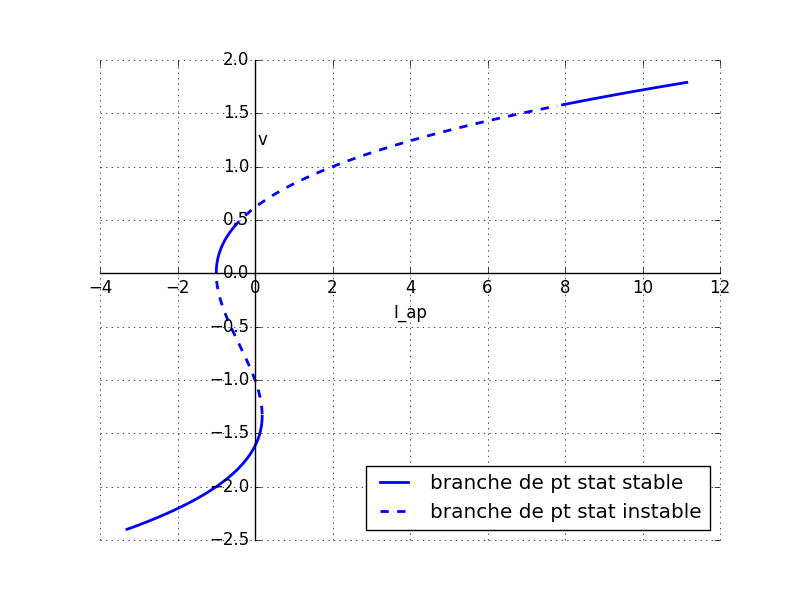
\includegraphics[width=0.6\textwidth]{bif2.png}
\end{center}
\end{frame}



\begin{frame}
\begin{align*}
\det(J_{(v)} - \lambda I_2)&=
\begin{vmatrix}
{\frac{-3v_0}{c}(v_0-2) -\lambda} & {\frac{1}{c}} \\ -10v_0 & -1 - \lambda \end{vmatrix} \\
	 &= \lambda^2 + \left(\frac{3}{c}v_0^2-\frac{6}{c}v_0 + 1\right)\lambda + \left(\frac{3}{c}v_0^2 + \frac{4}{c}v_0\right)  \\
	 \Delta & =  \left(\frac{3v_0}{c}(v_0 - 2) + 1\right)^2 - 4\frac{v_0}{c}(4 + 3v_0) \\
	 & = \frac{9v_0^4}{c^2} - \frac{36v_0^3}{c^2} + \frac{6}{c}(\frac{6}{c} - 1)v_0^2 - \frac{28v_0}{c} + 1
\end{align*}
\end{frame}





\begin{frame}{Bifurcation pli (col-n\oe ud)}
\begin{itemize}
\item Le determinant de la jaconienne s'annule.
\item 2 nouvelles branches de points stationnaires apparaissent
Interprétation avec le diagramme de bifurcation $I_{ap}= f(v_0)$
\end{itemize}



\only<3>{
\begin{align*}
\frac{df}{dv_0} &= 0  \\
3v_0^2 + 4v_0 &= 0\\
v_0(3v_0 + 4) &= 0
\end{align*}

Il y a 2 bifurcations pli: $v=0$ et $v=-4/3$.}


\only<2>{
Dans cette dernière représentation, les points de bifurcation pli correspondent à des extrema locaux de la fonction $f$.
\begin{center}
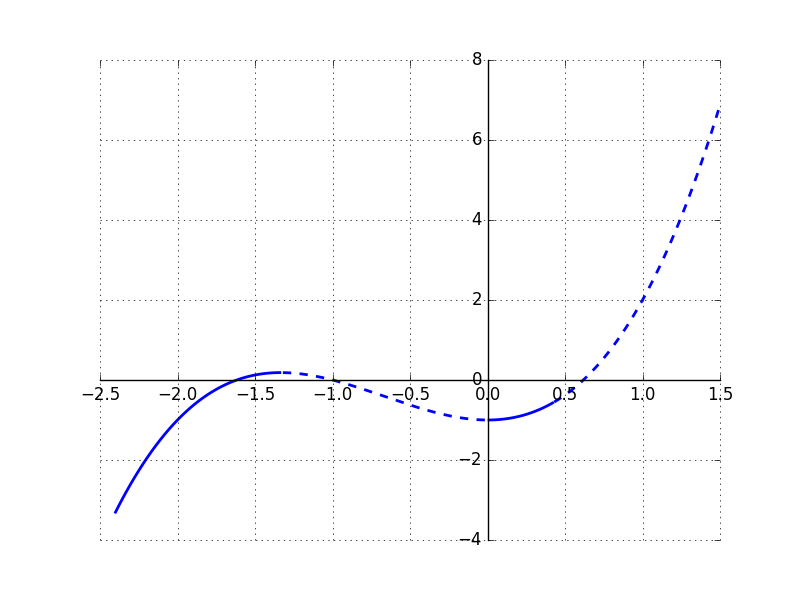
\includegraphics[height=0.3\textwidth]{bif_retourne}
\end{center}}



\end{frame}

\begin{frame}
\begin{center}
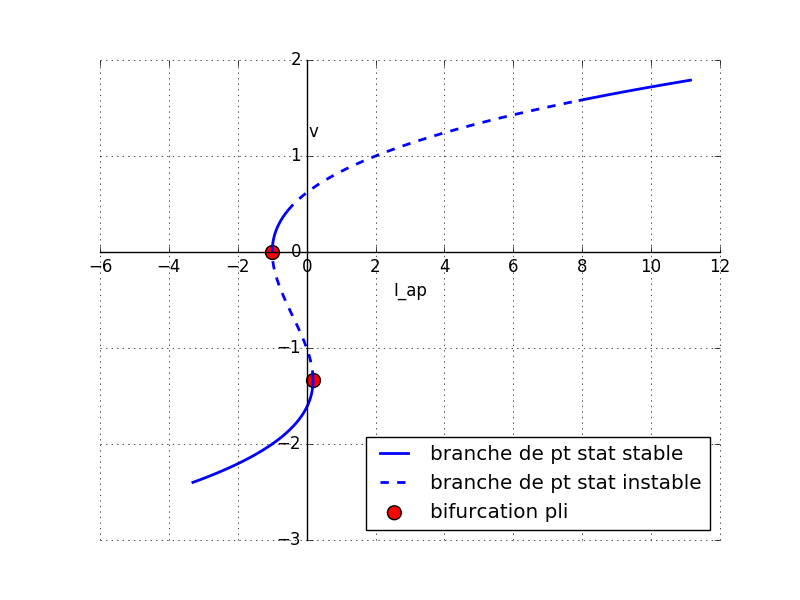
\includegraphics[width=0.6\textwidth]{bif3.png}
\end{center}
\end{frame}

\begin{frame}{Bifurcation de Hopf}
\begin{itemize}
\item un foyer stable devient un foyer instable
\item un cycle limite stable apparait\\
\item les conditions à vérifier :
\begin{itemize}
\item $v < v_H$ : foyer stable ou instable
\item $v > v_H$ : foyer avec la stabilité opposée
\item $\left.\dfrac{dRe(\lambda)}{dI_{ap}}\right|_{v_H} \ne 0$ $\Leftrightarrow$ $\left.\dfrac{d\left(\frac{3v_0}{2c}((2-v_0) - 1)\right)}{dI_{ap}}\right|_{v_H} \ne 0$
\end{itemize}
\item<2> Il y a 2 bifurcations de Hopf : $v = 1 -\frac{\sqrt(3)}{3}$ et  $v = 1 +\frac{\sqrt(3)}{3}$
\end{itemize}
\end{frame}

\begin{frame}
\begin{center}
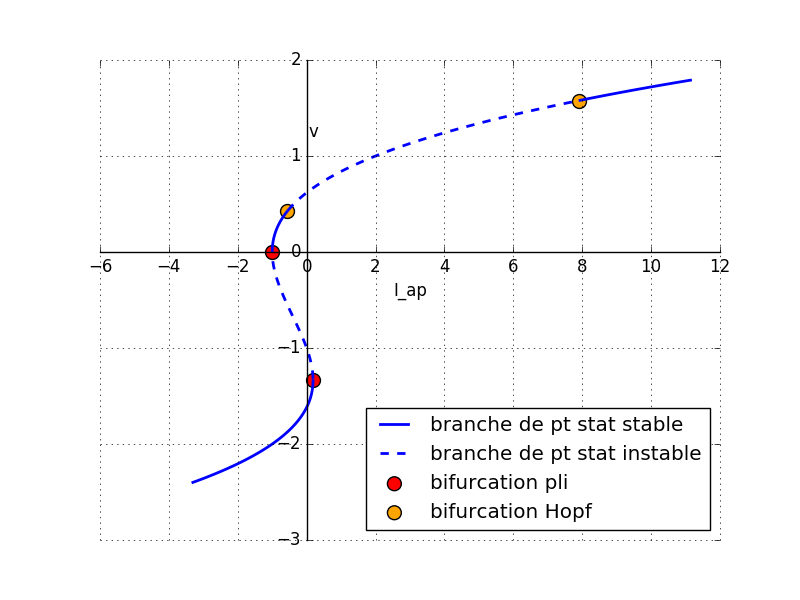
\includegraphics[width=0.6\textwidth]{bif4.png}
\end{center}
\end{frame}


\begin{frame}
 \only<1>{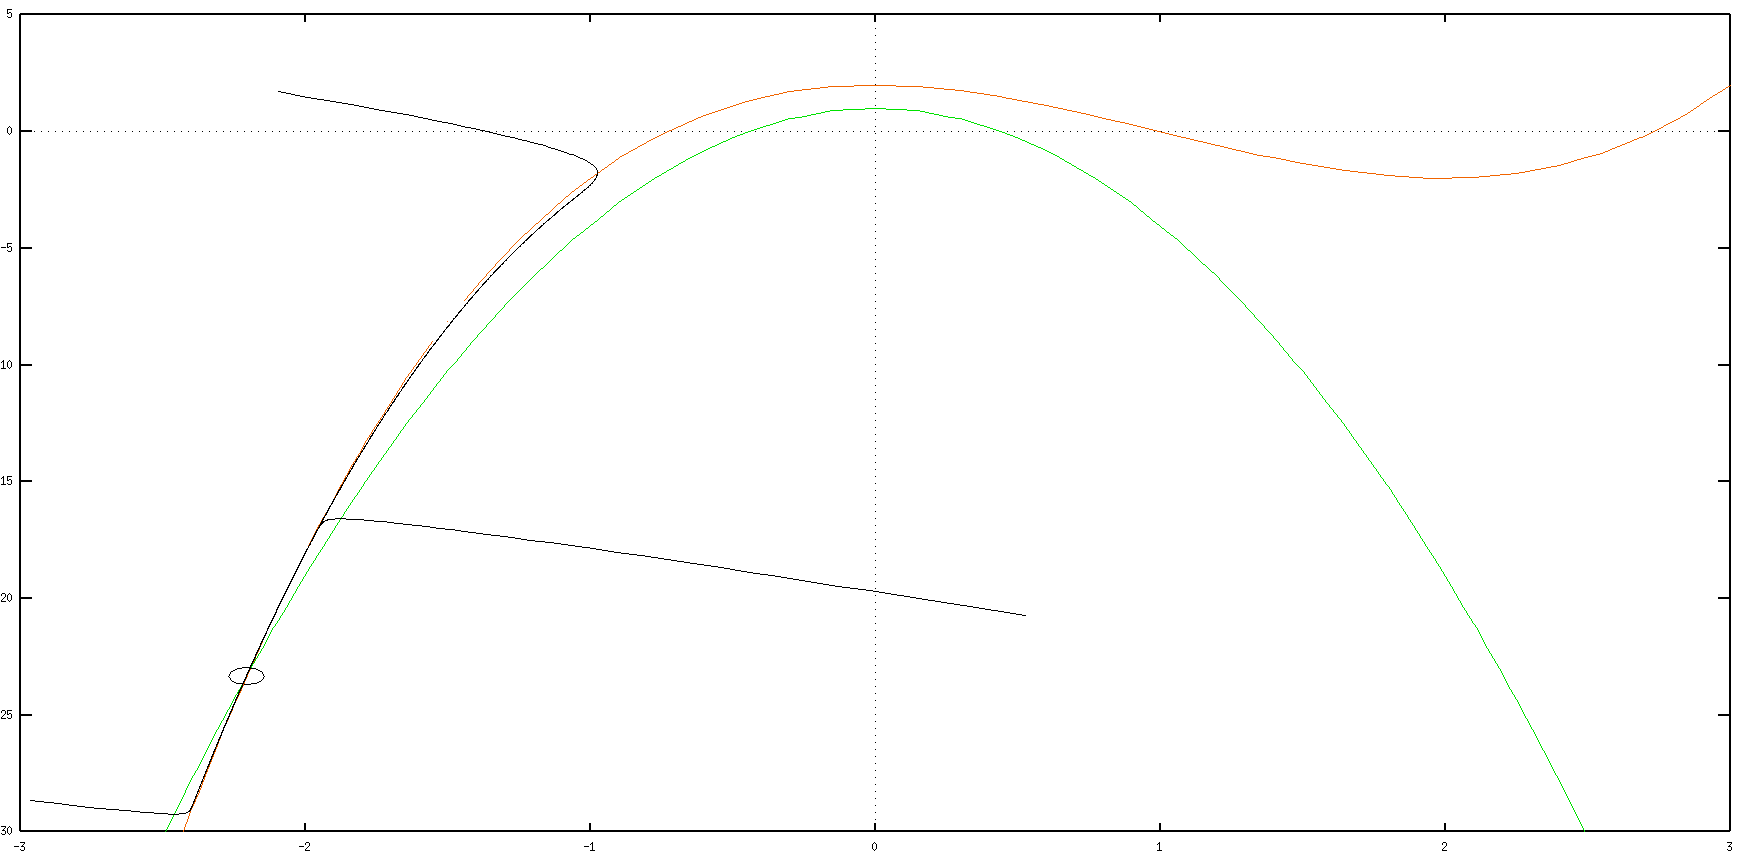
\includegraphics[height=5cm]{I_000} }
  \only<2>{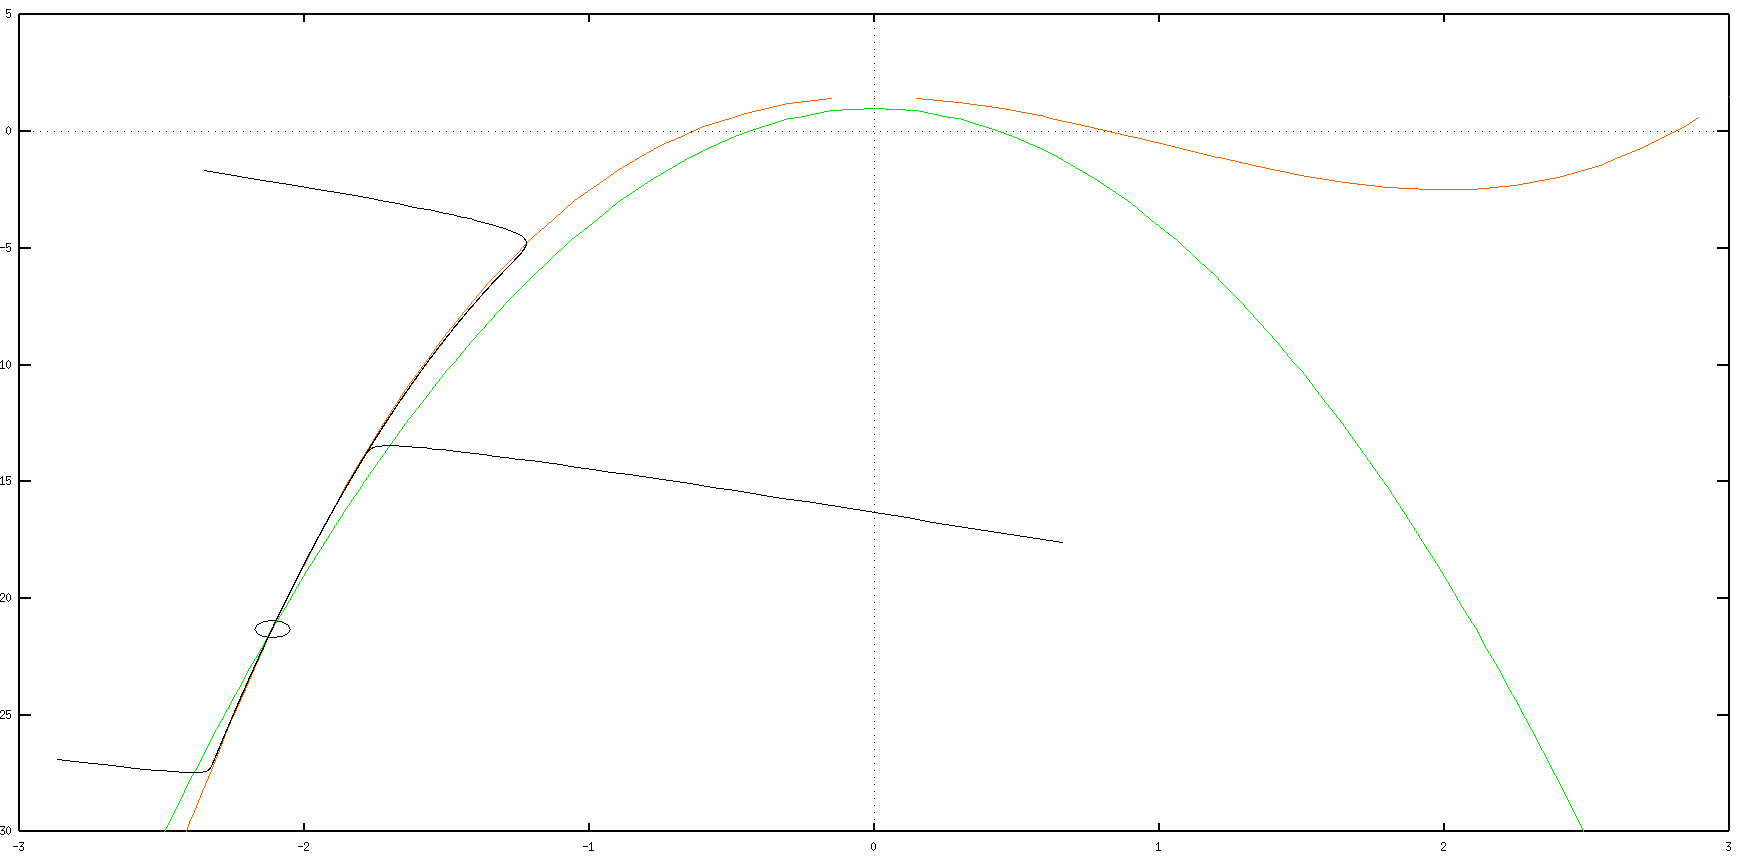
\includegraphics[height=5cm]{I_001}}
  \only<3>{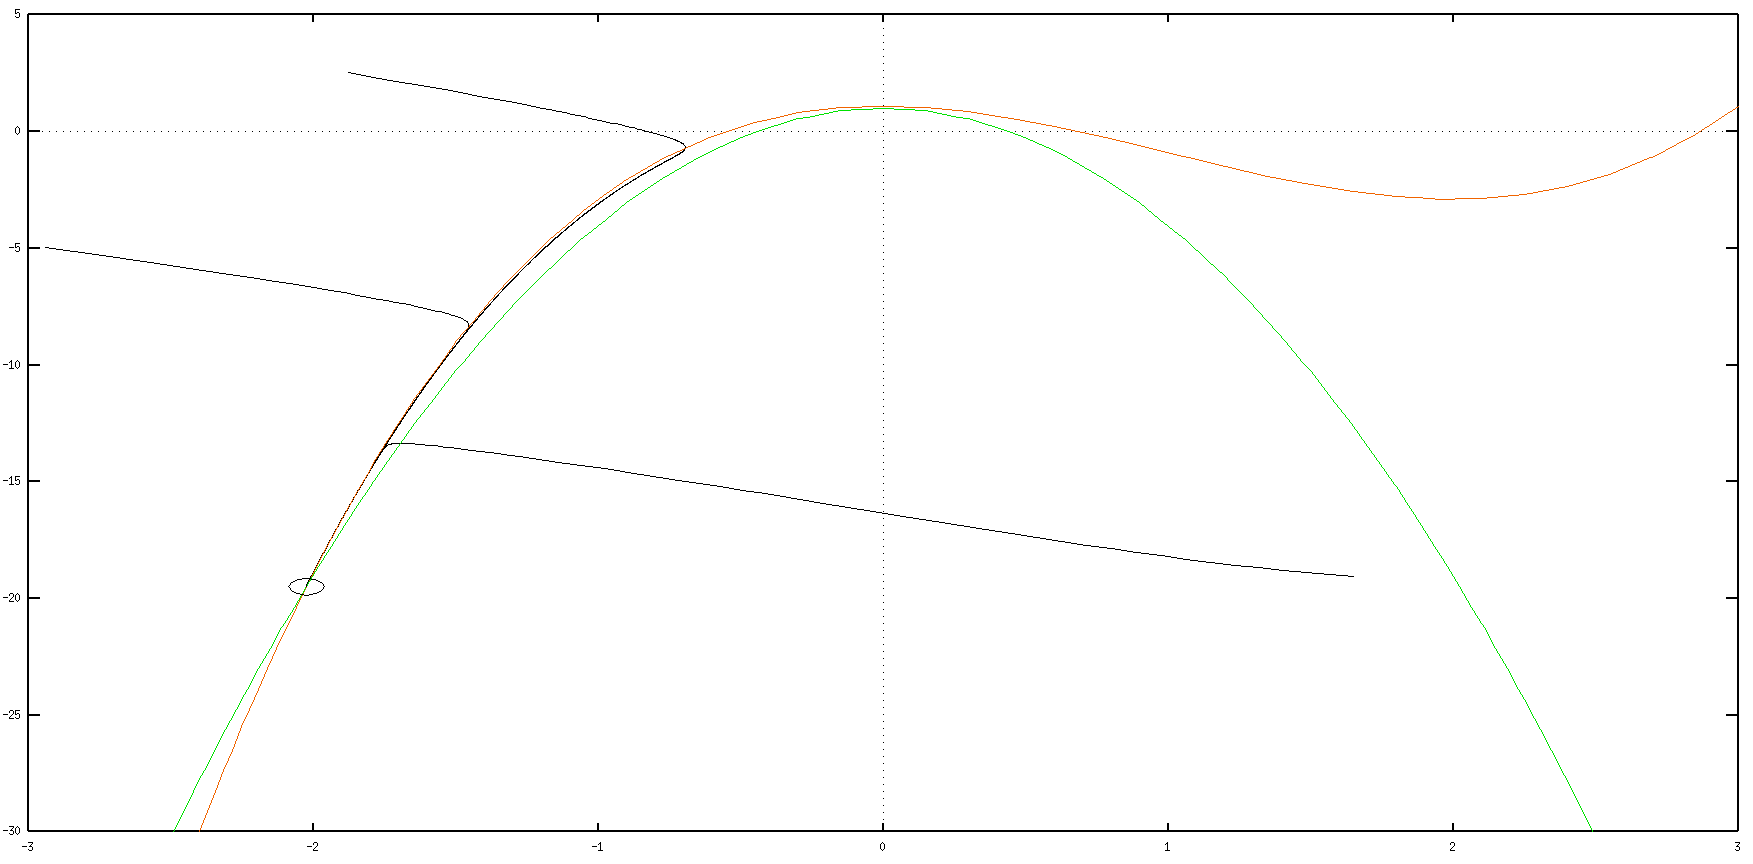
\includegraphics[height=5cm]{I_002}}
   \only<4>{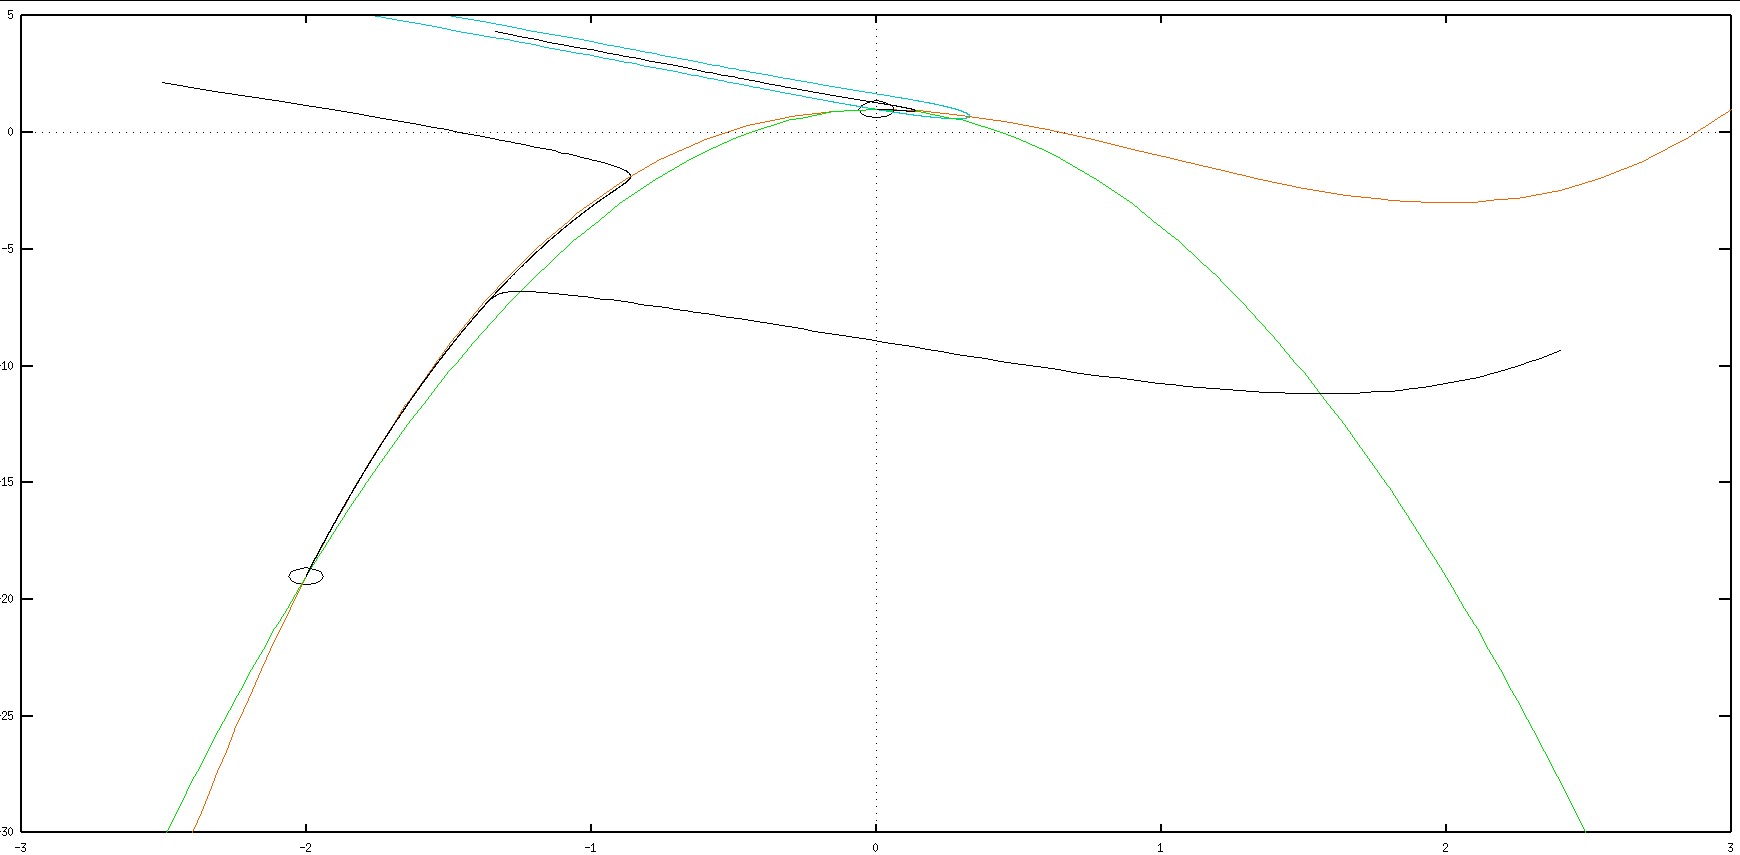
\includegraphics[height=5cm]{I_003}}
    \only<5> {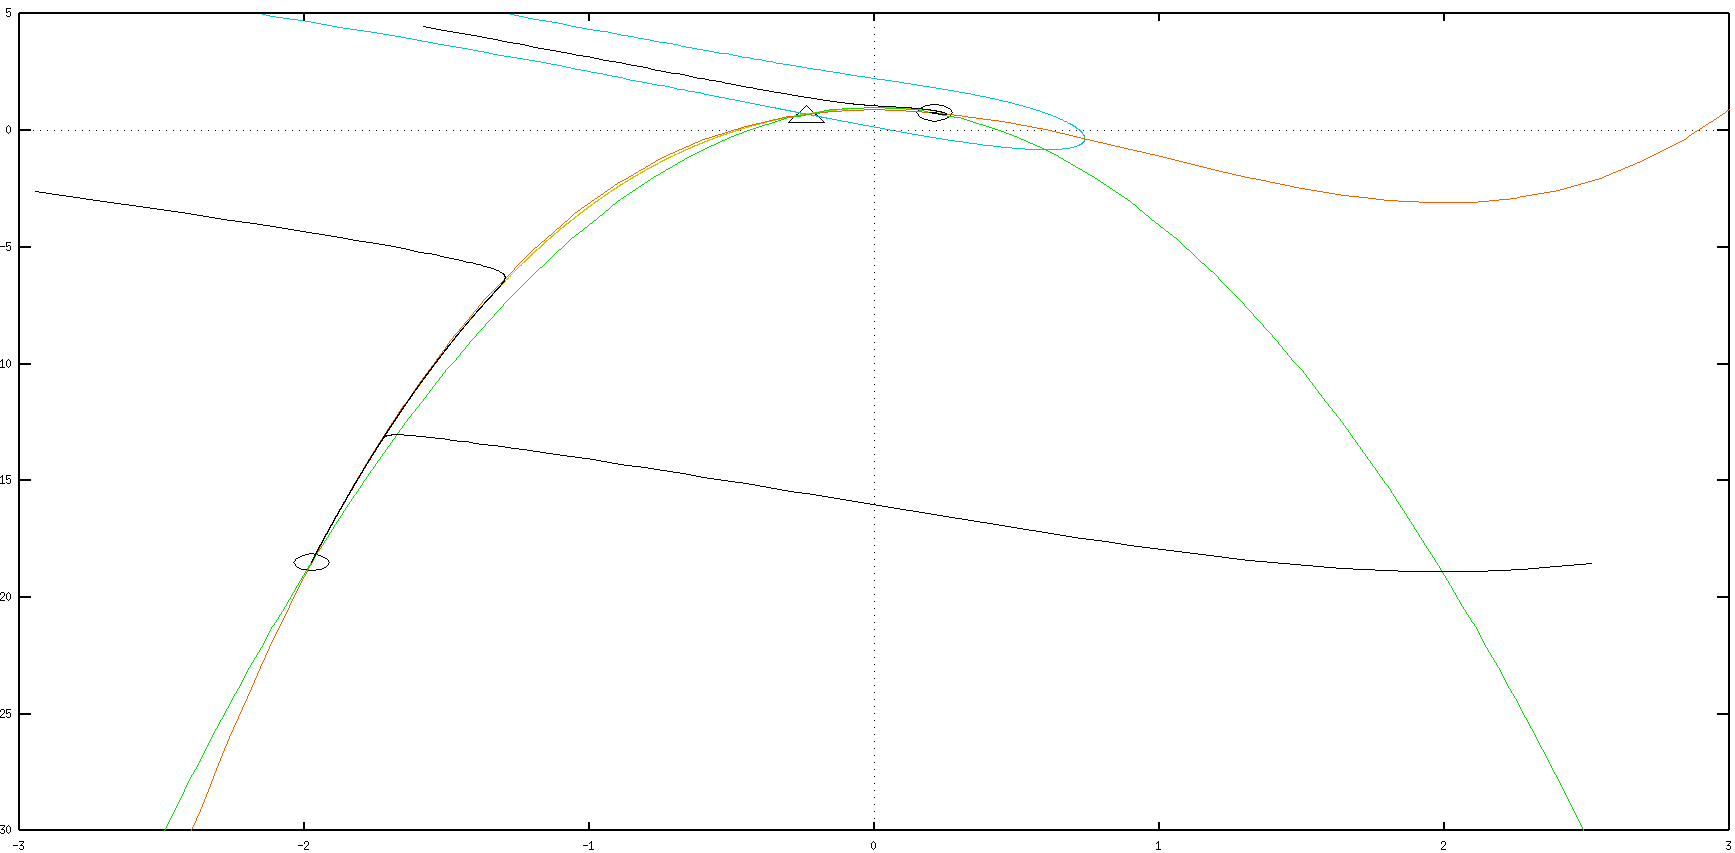
\includegraphics[height=5cm]{I_004}}
 \only<6> {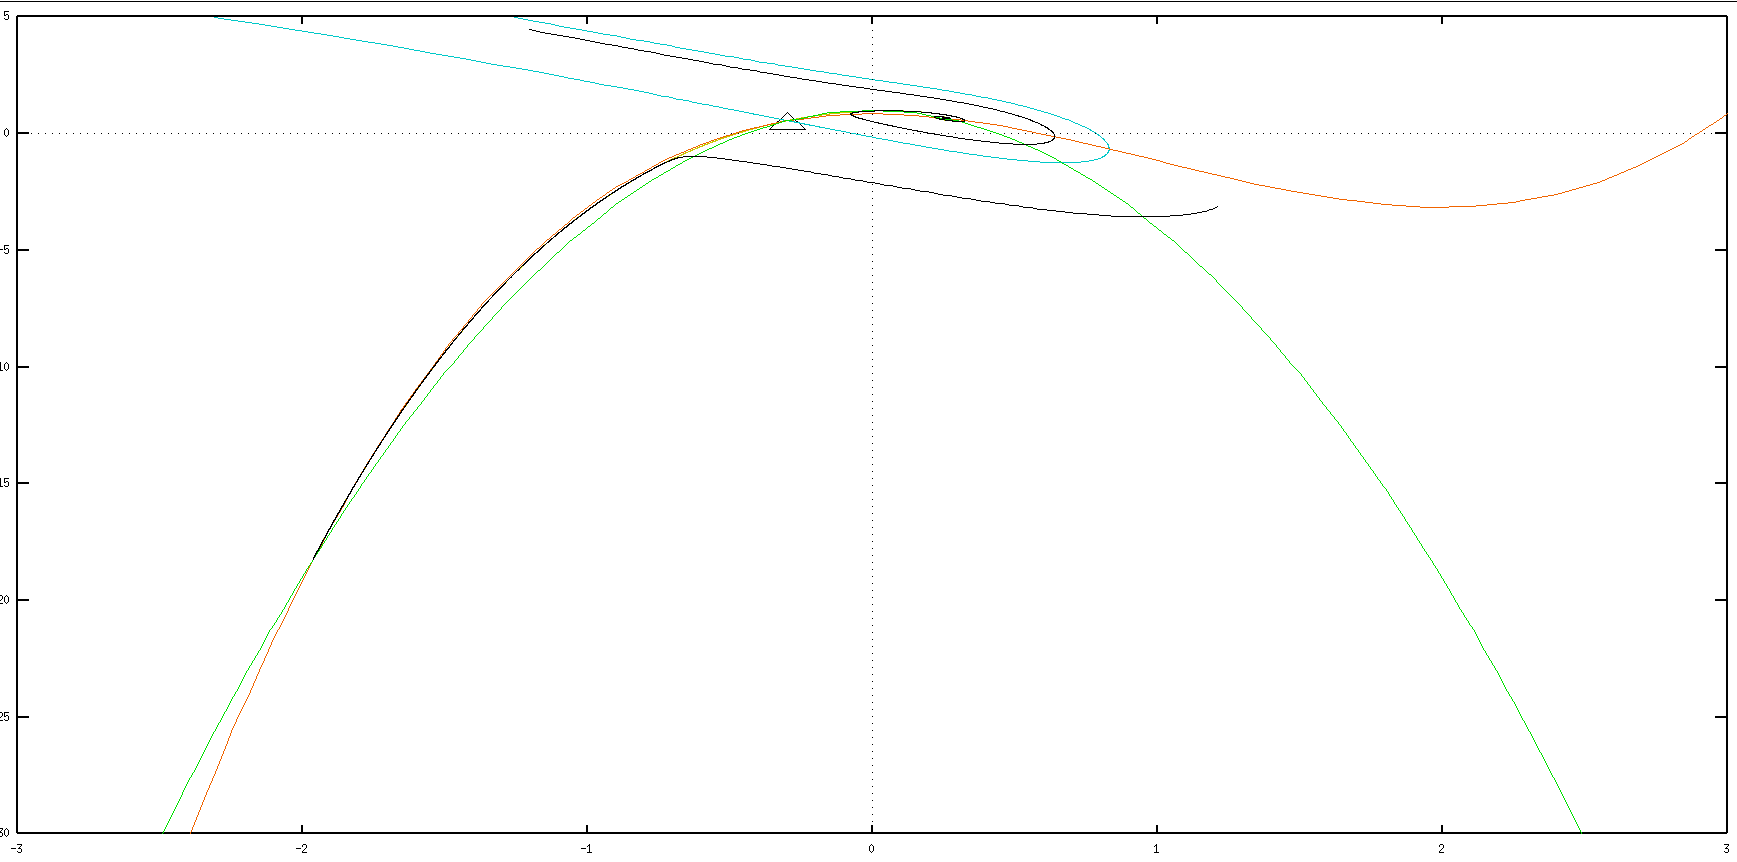
\includegraphics[height=5cm]{I_005}}
 \only<7> {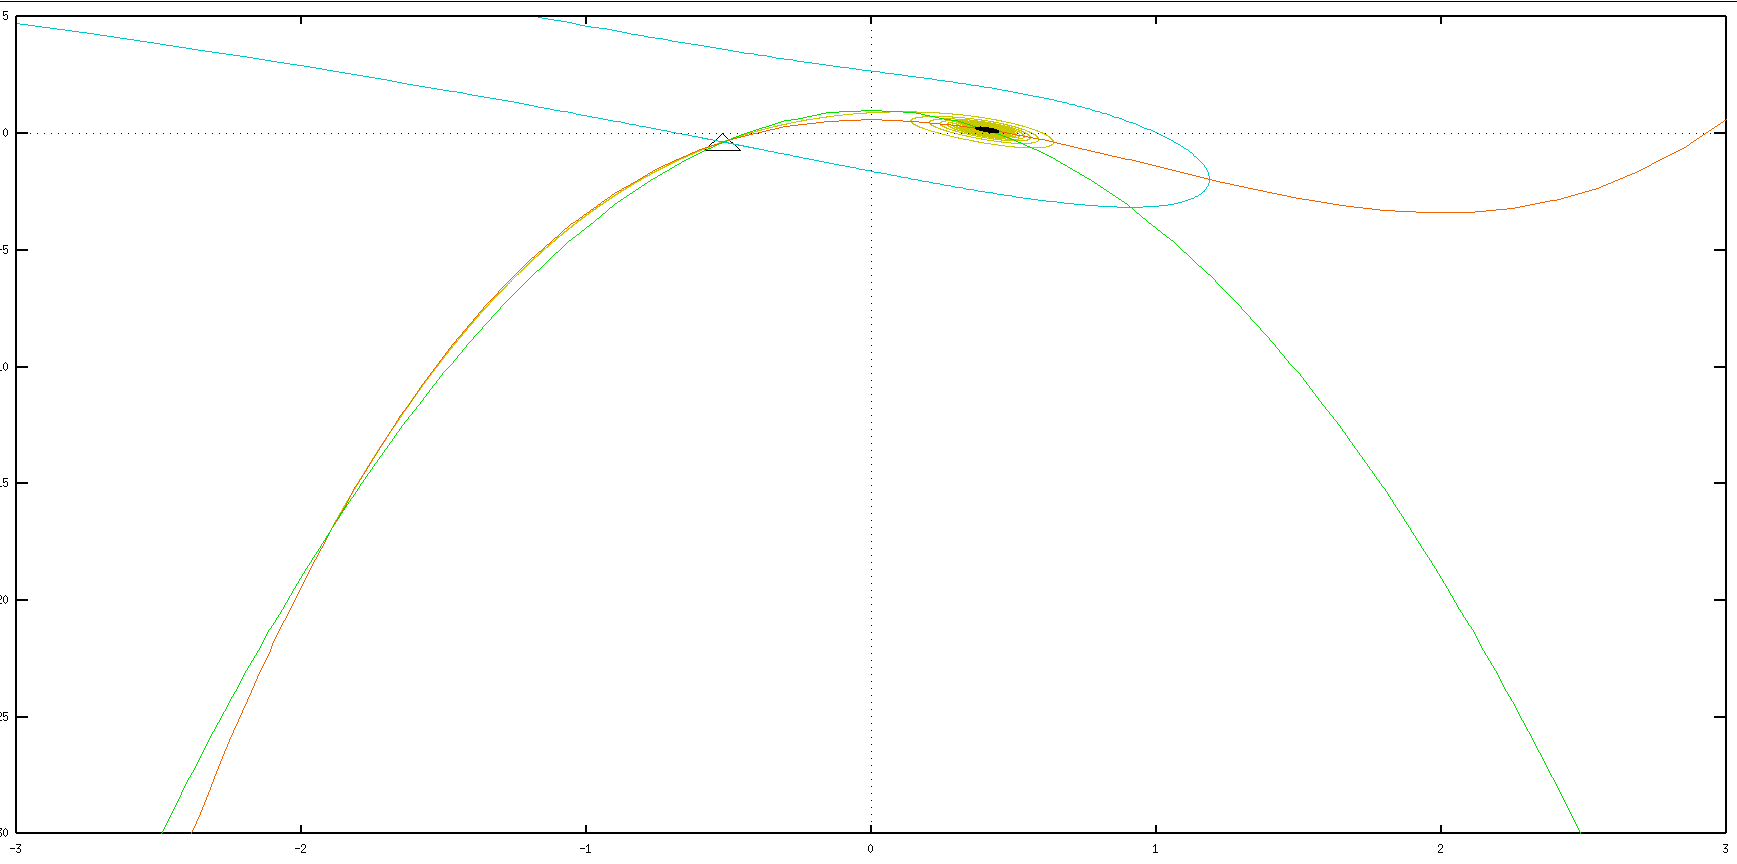
\includegraphics[height=5cm]{I_006}}
  \only<8>{ 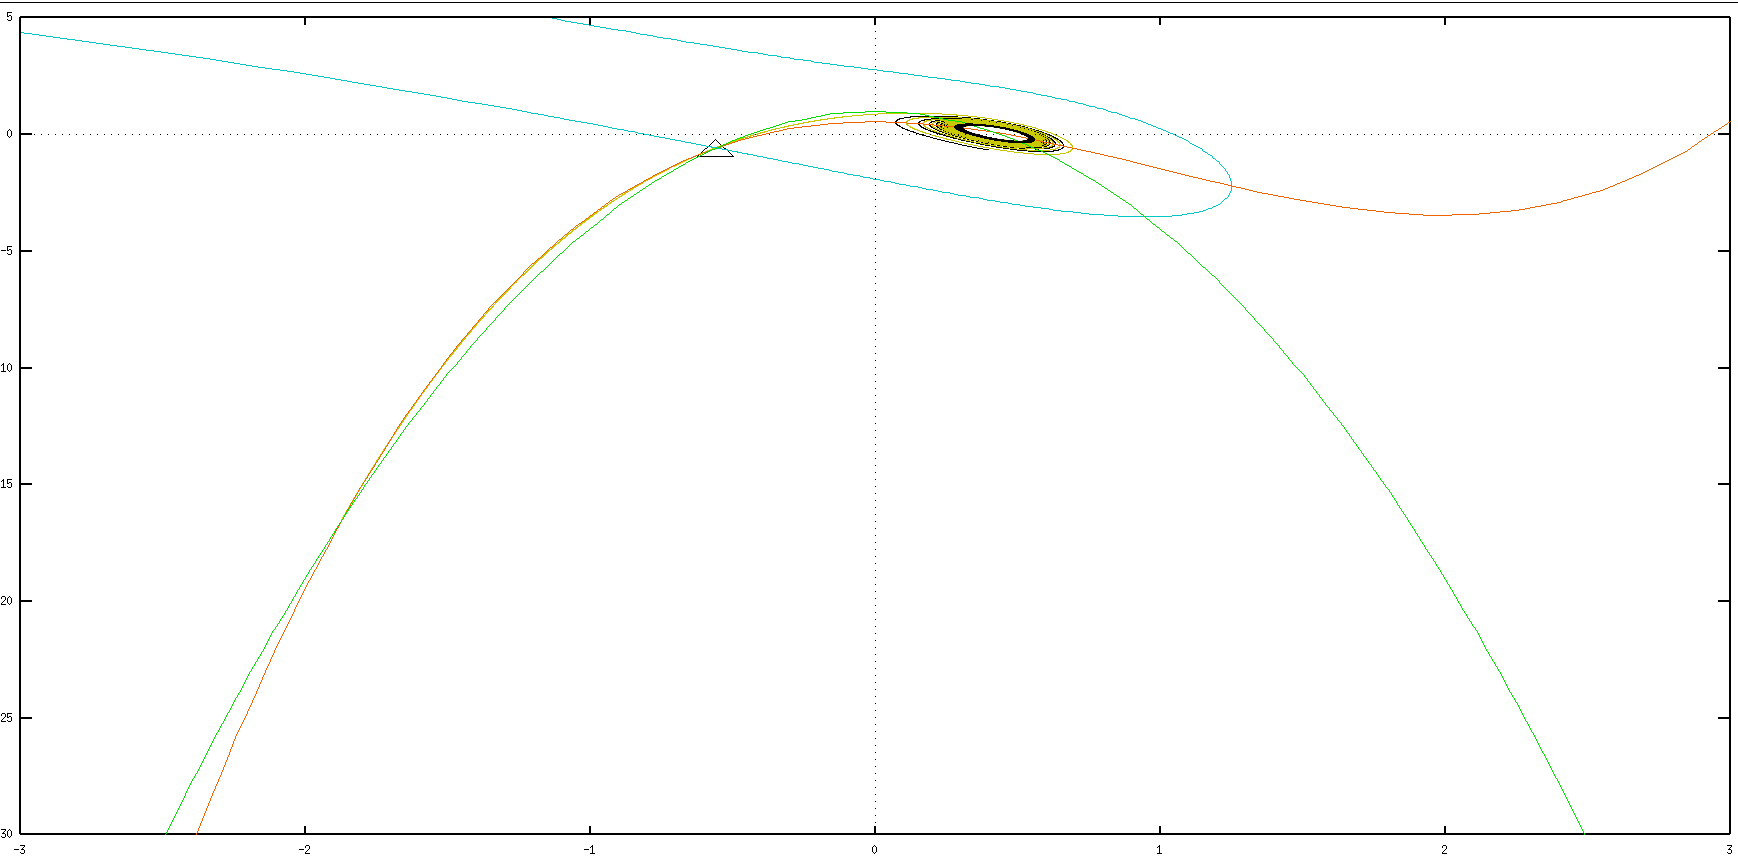
\includegraphics[height=5cm]{I_007}}
  \only<9> {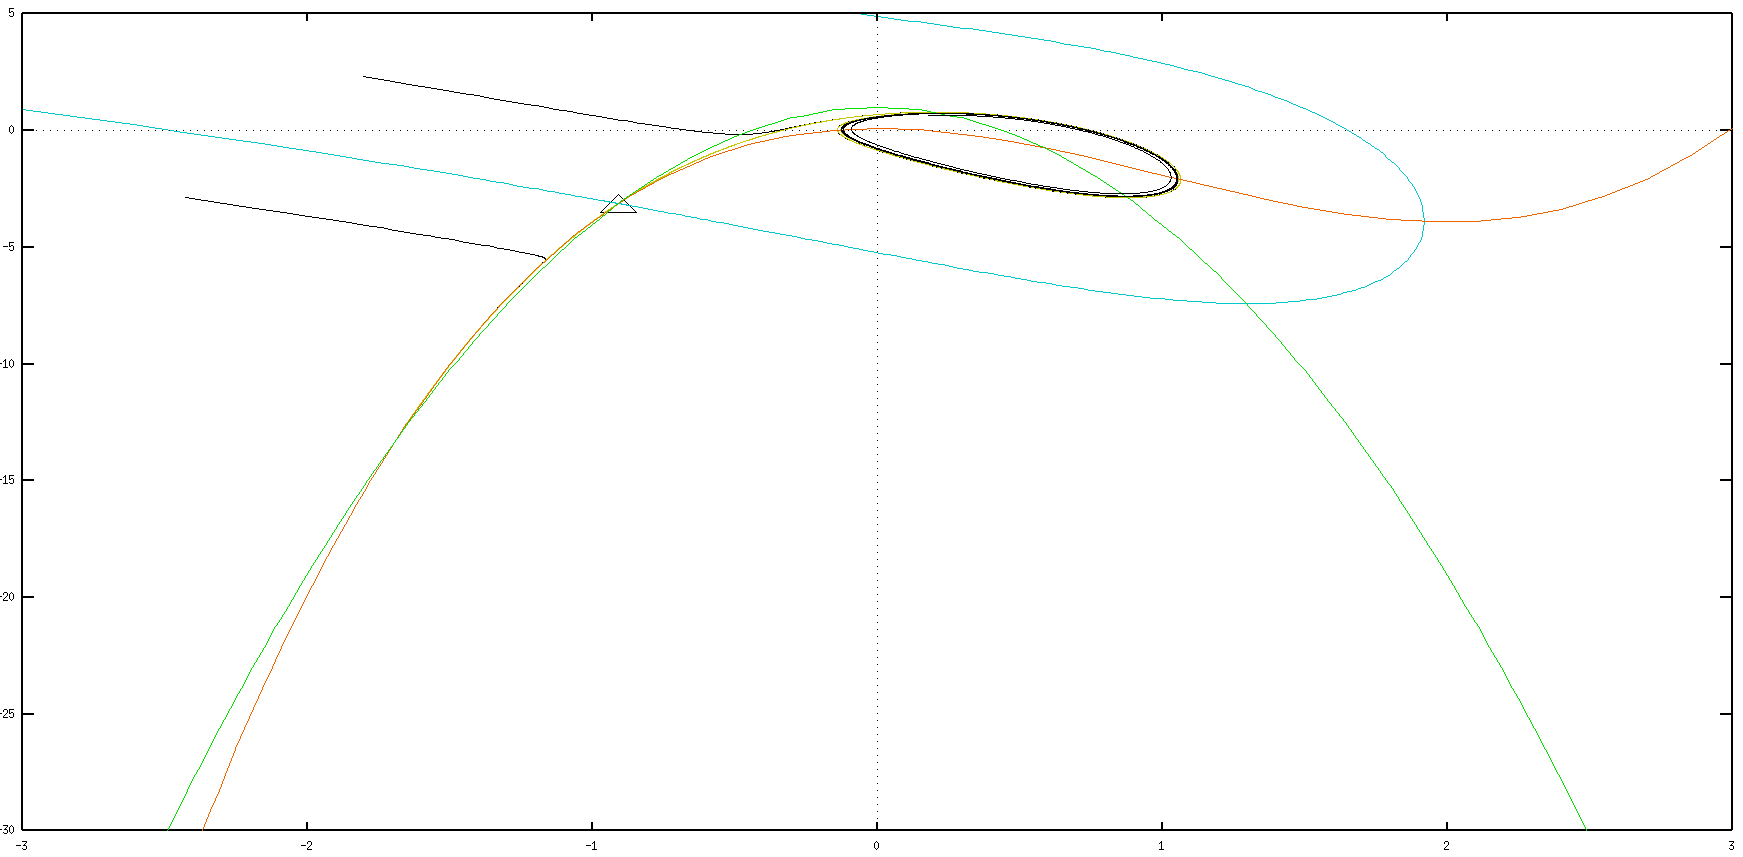
\includegraphics[height=5cm]{I_008}}
    \only<10> {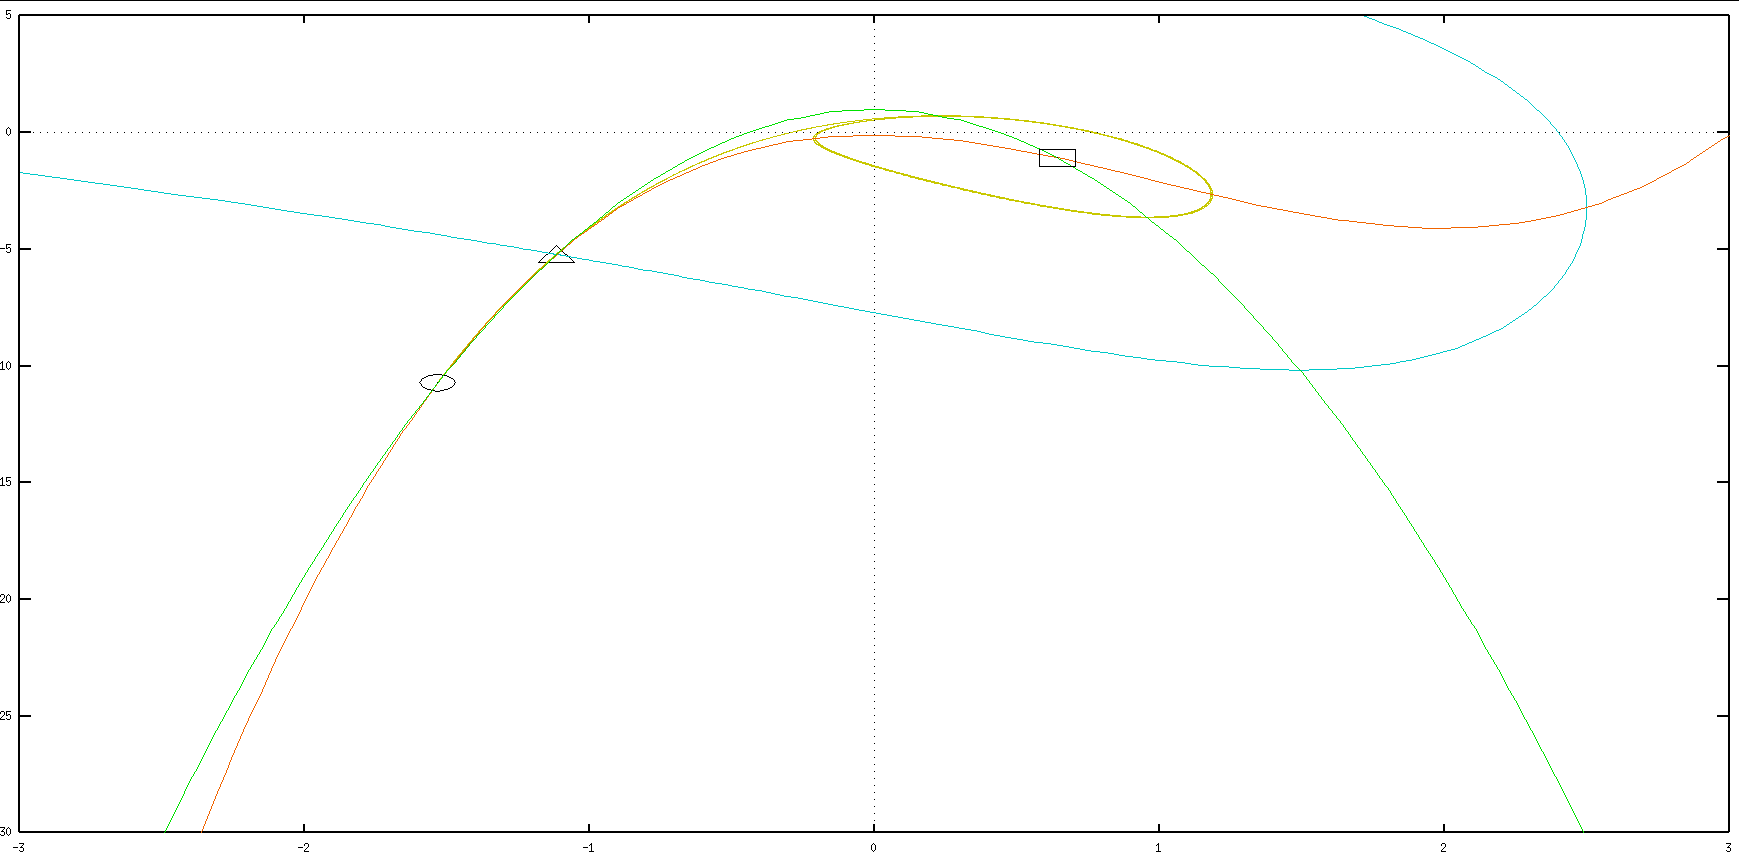
\includegraphics[height=5cm]{I_009}}
\only<11> {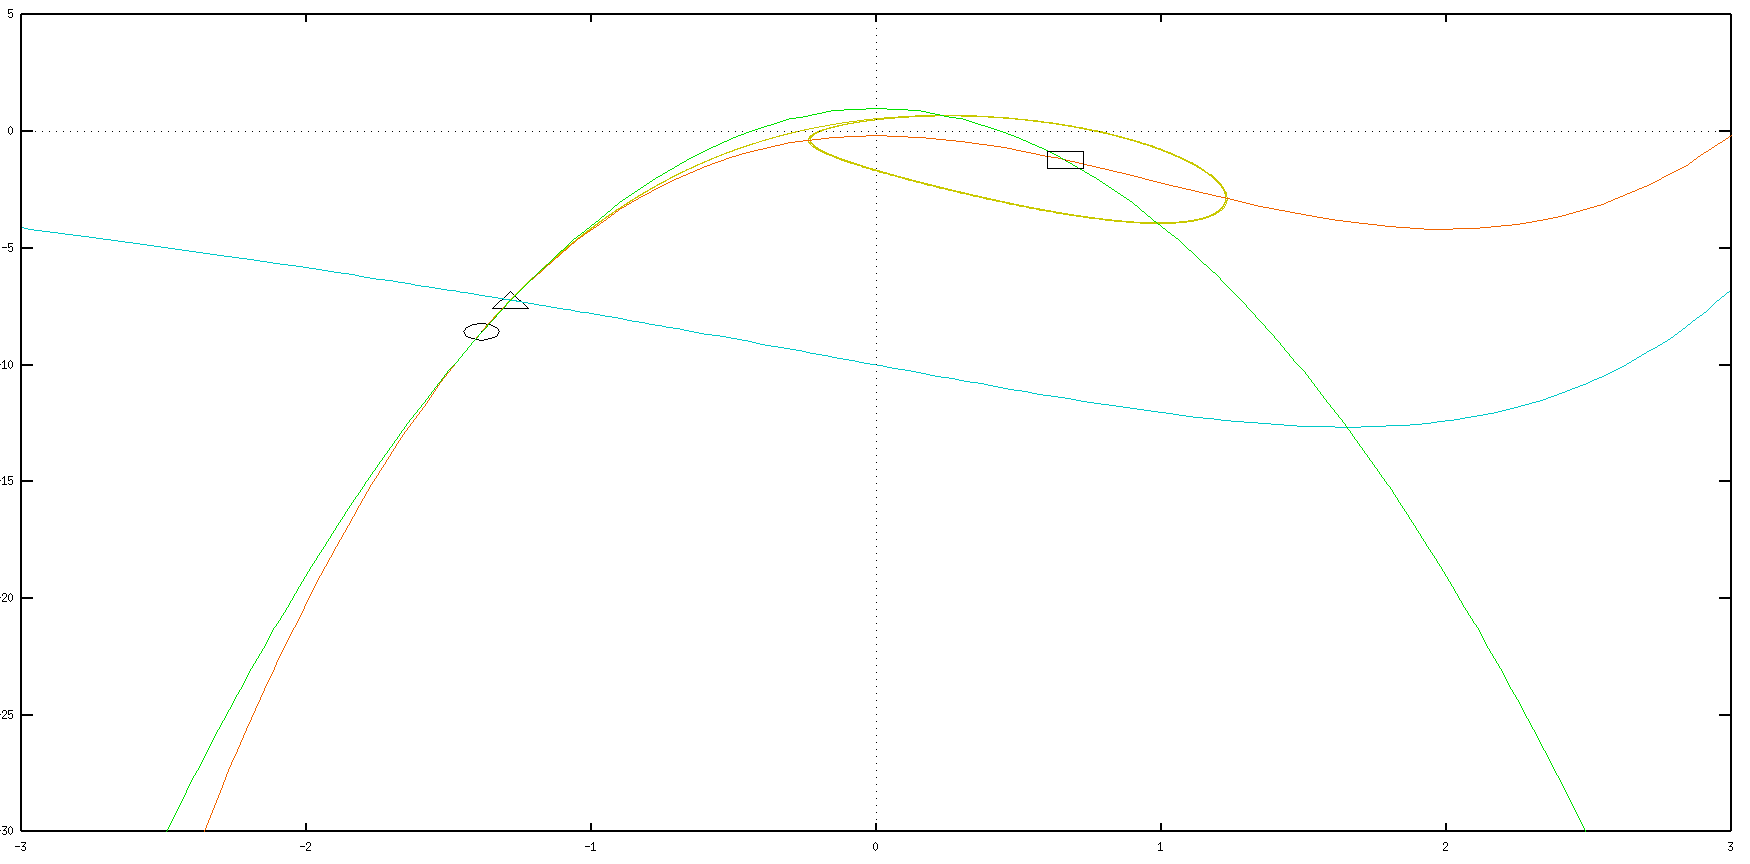
\includegraphics[height=5cm]{I_010}}
 \only<12> {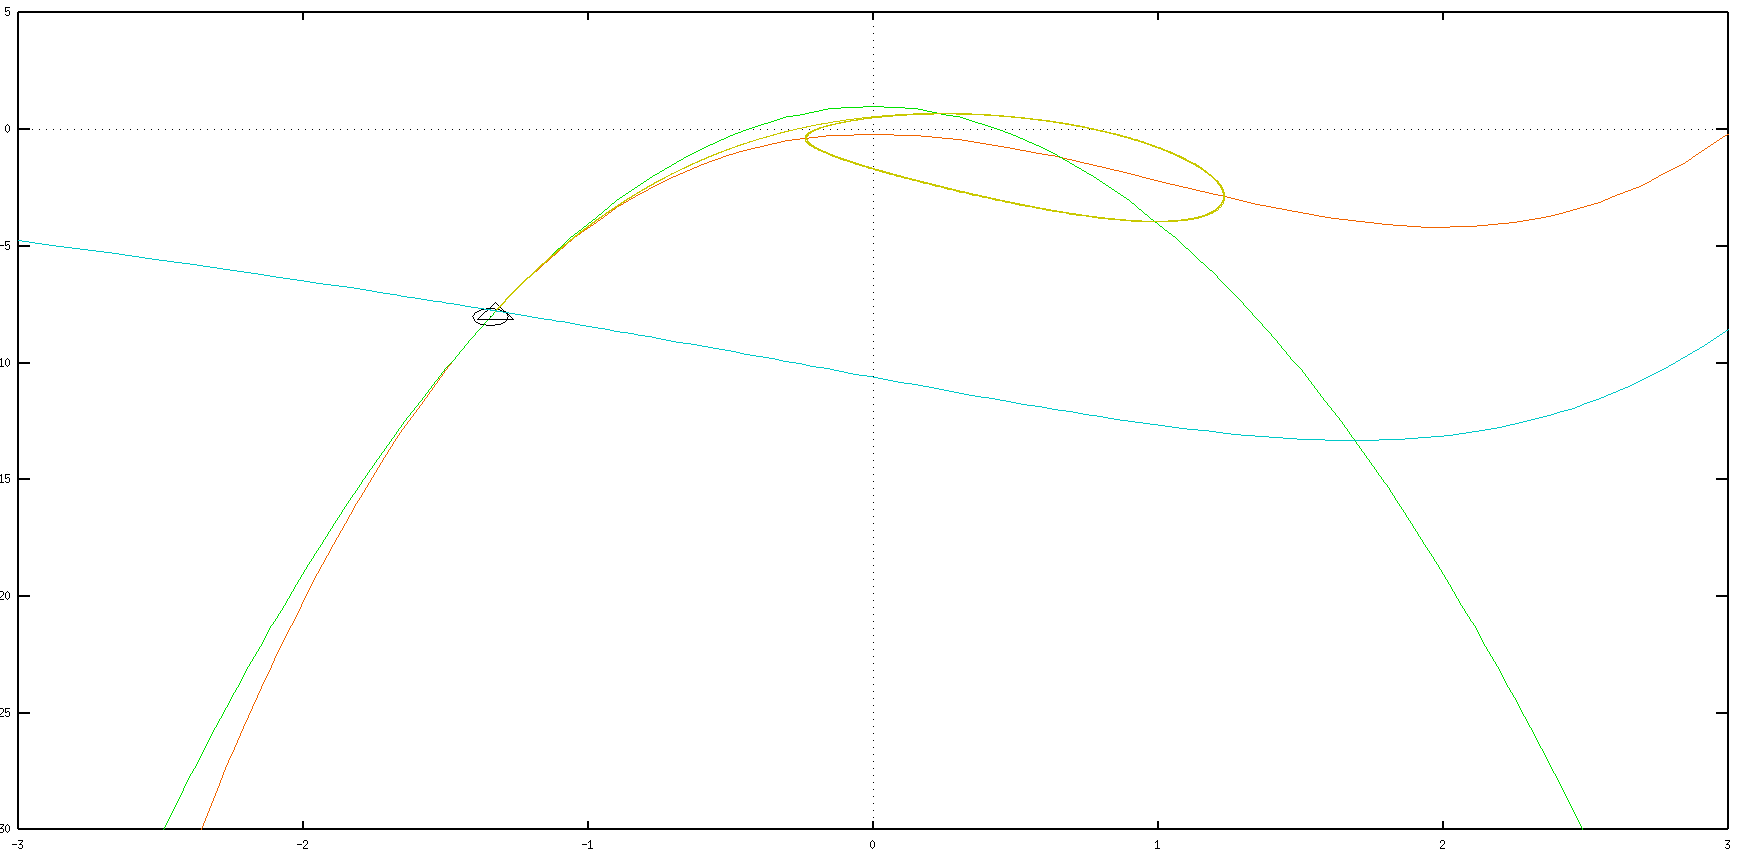
\includegraphics[height=5cm]{I_011}}
  \only<13> {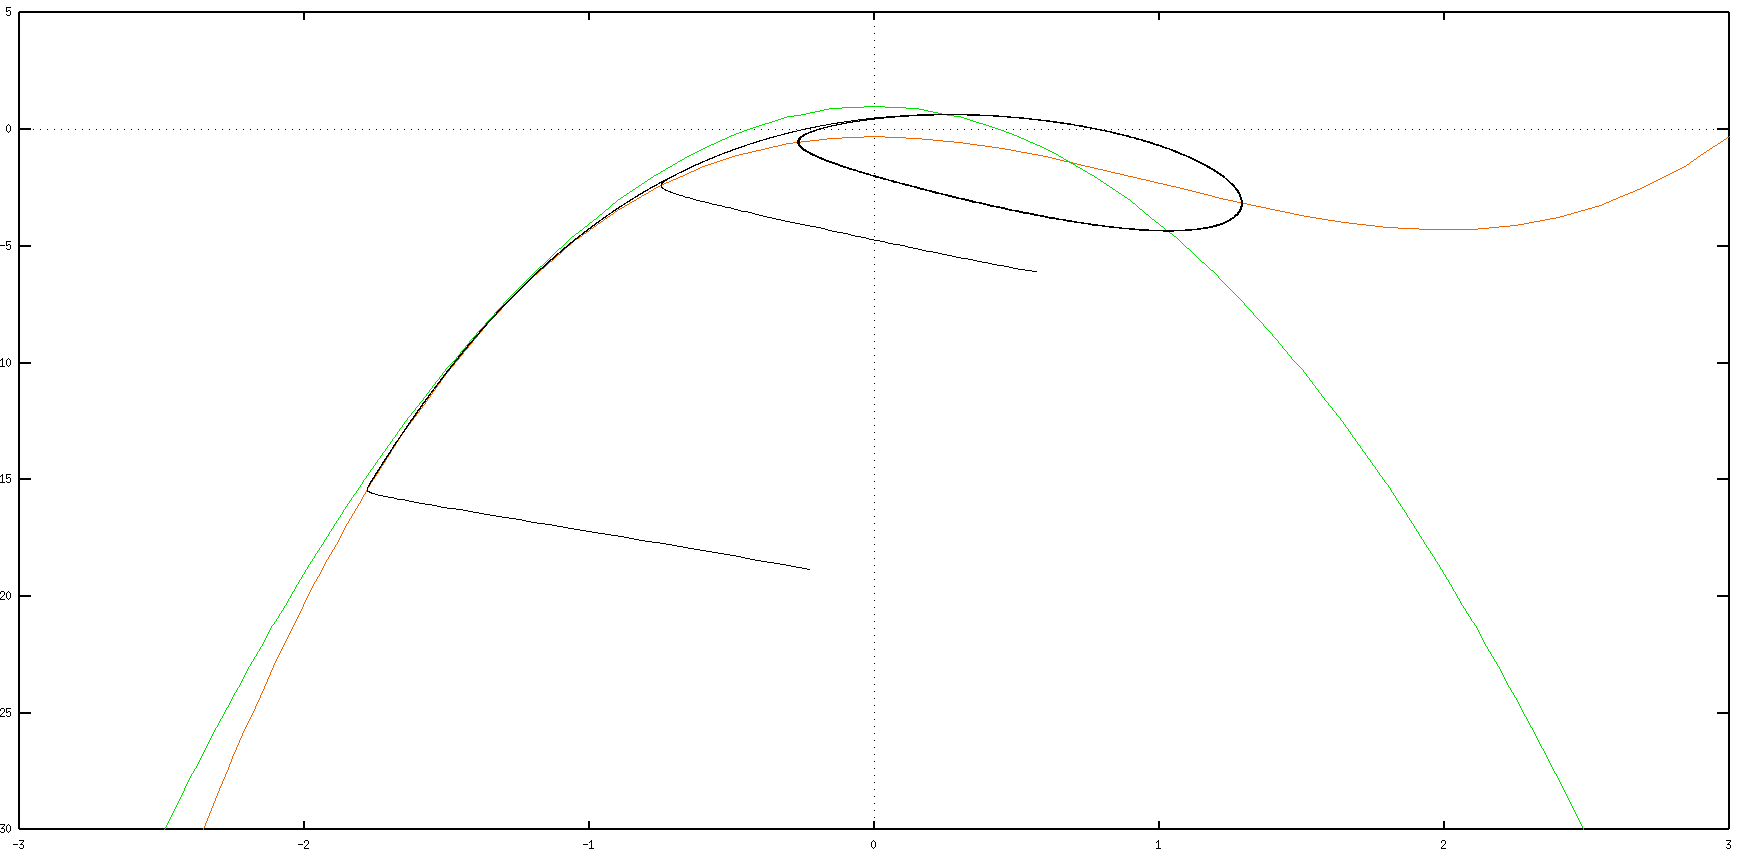
\includegraphics[height=5cm]{I_012}}
   \only<14> {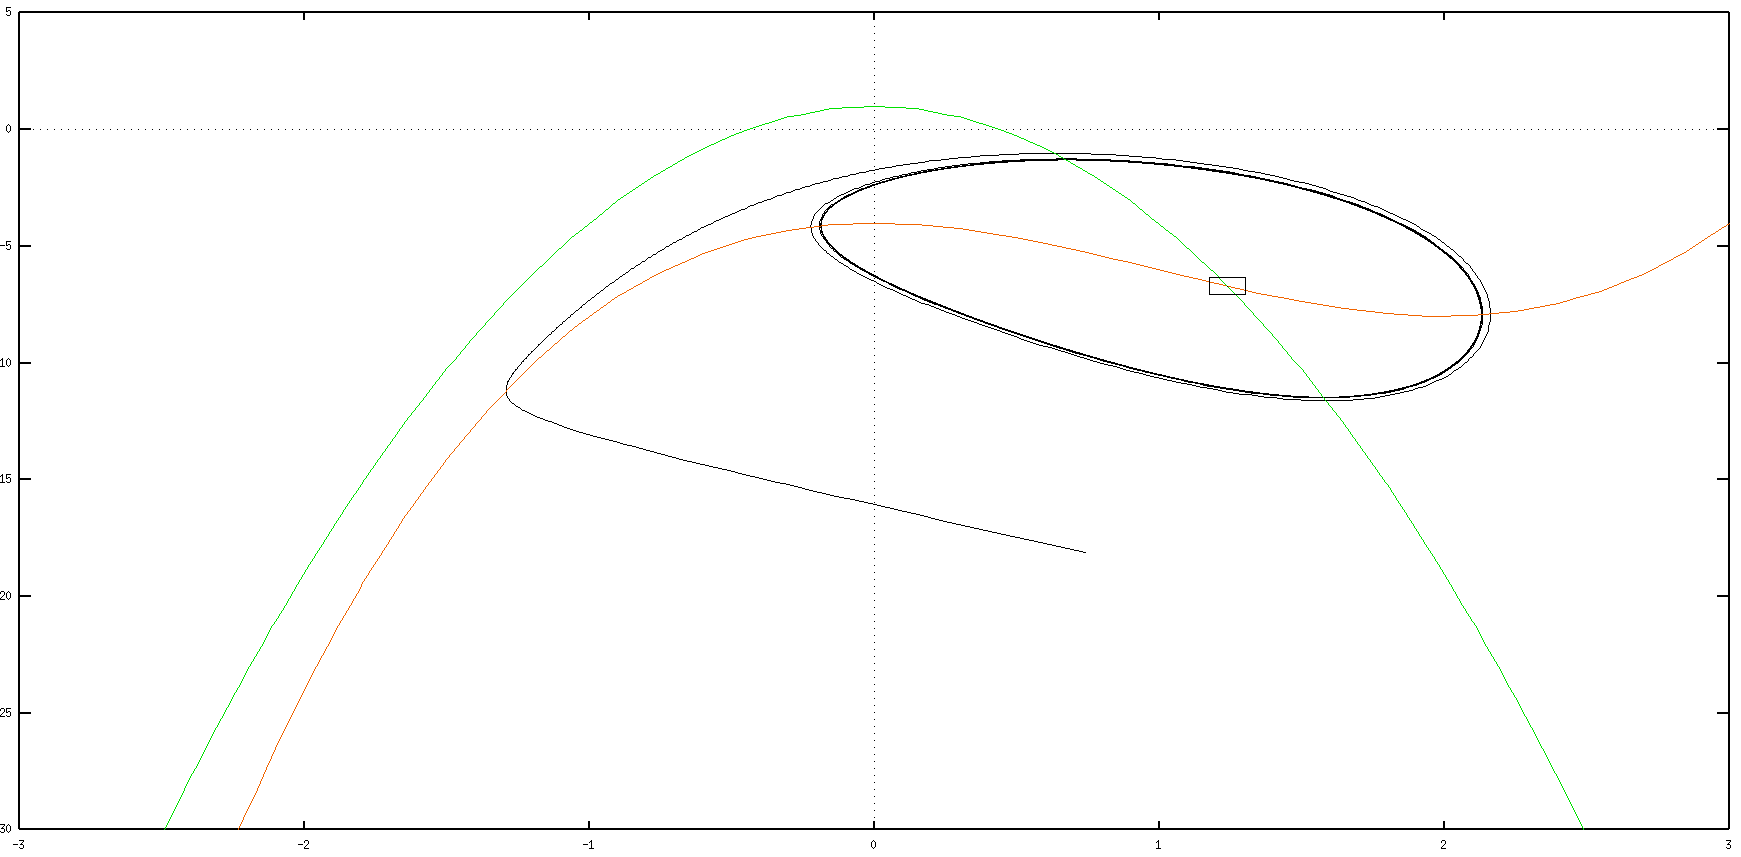
\includegraphics[height=5cm]{I_013}}
    \only<15> {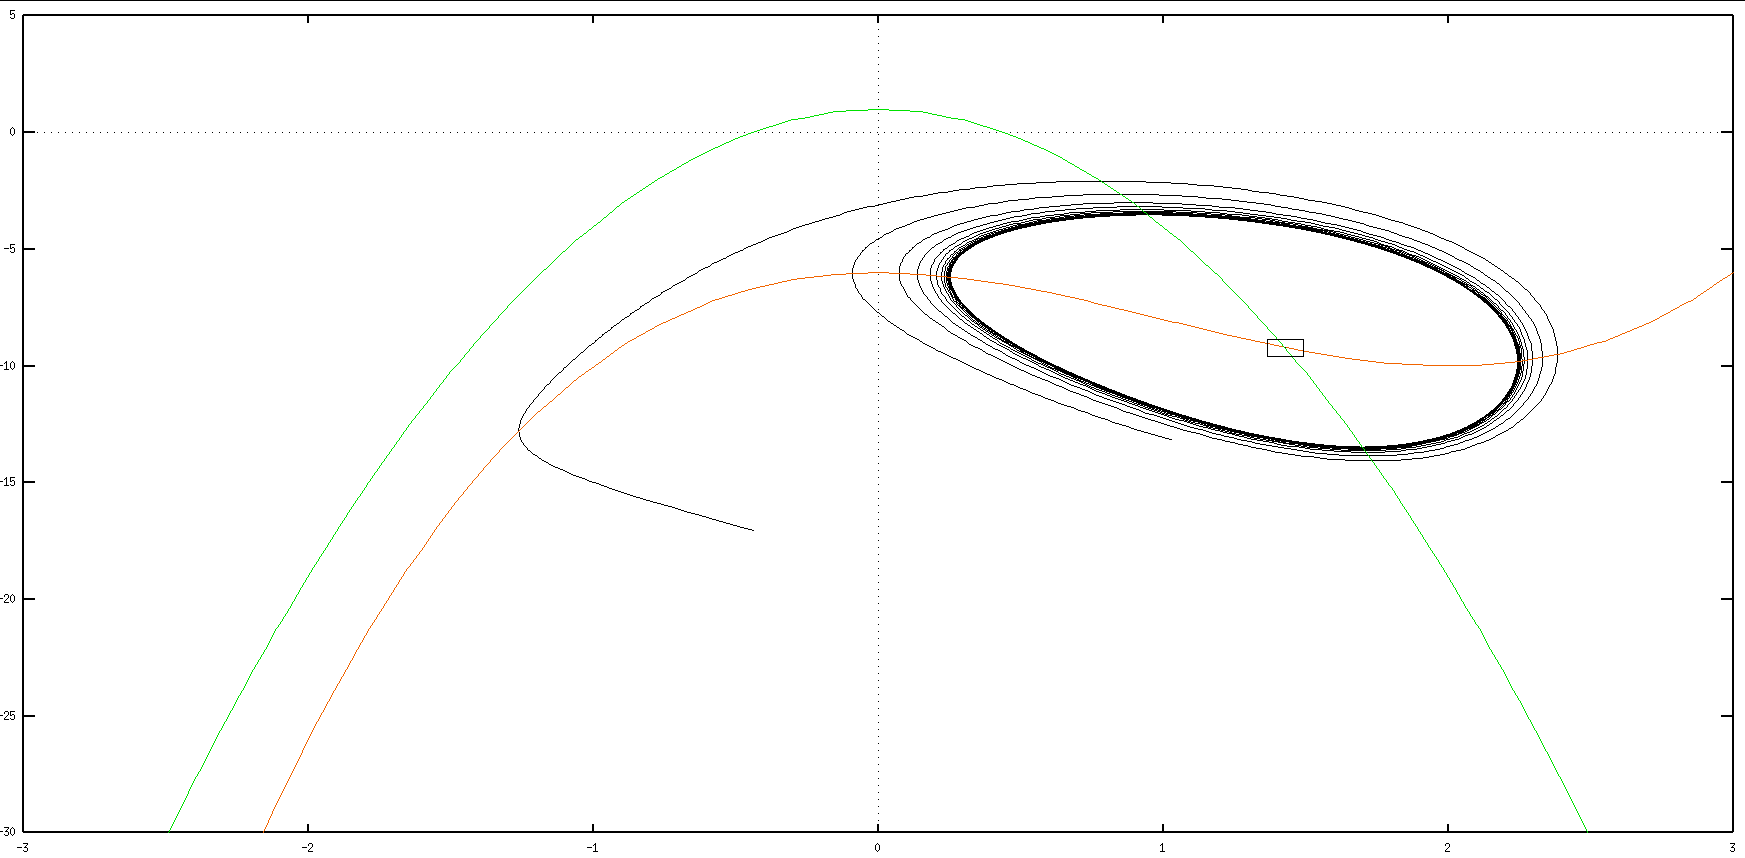
\includegraphics[height=5cm]{I_014}}
 \only<16> {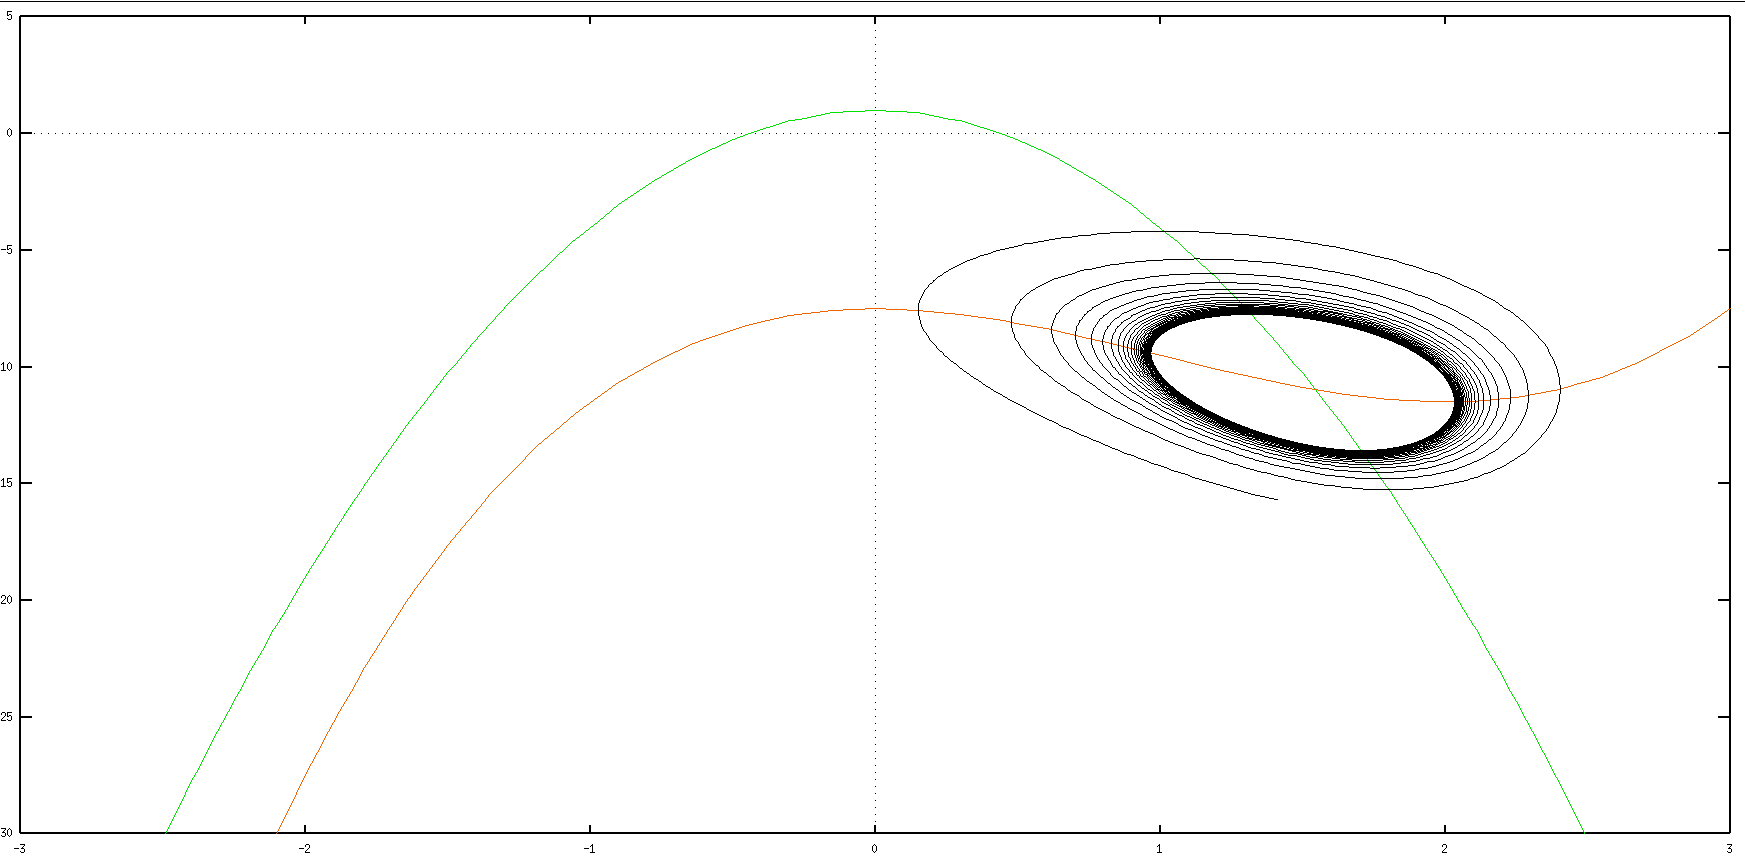
\includegraphics[height=5cm]{I_015}}
 \only<17> {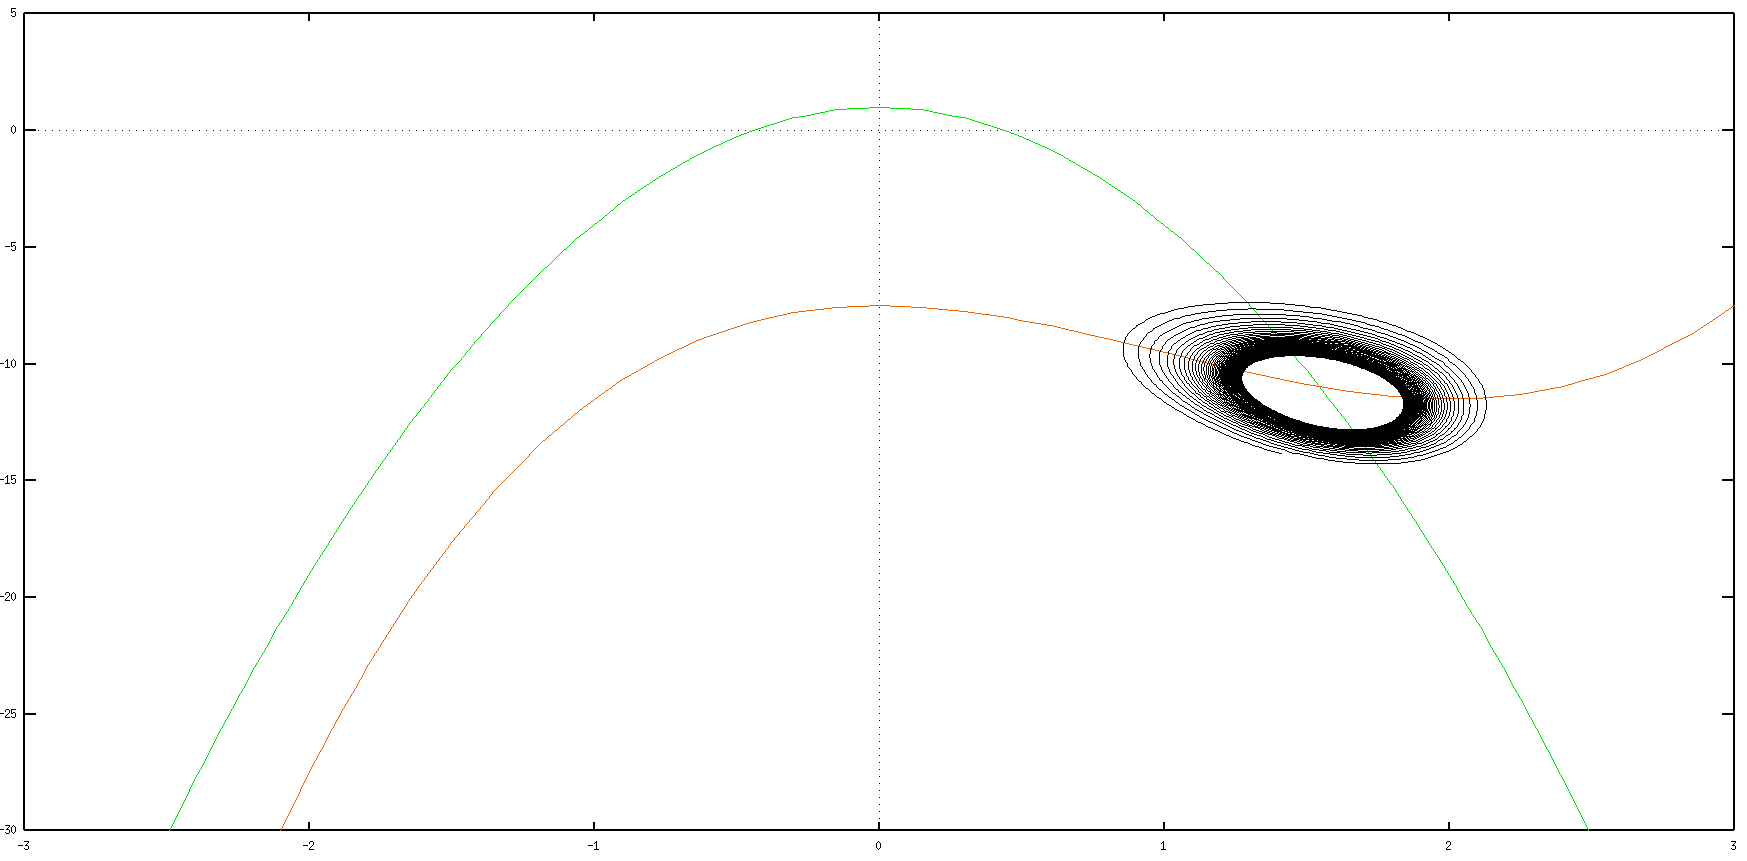
\includegraphics[height=5cm]{I_016}}
  \only<18> {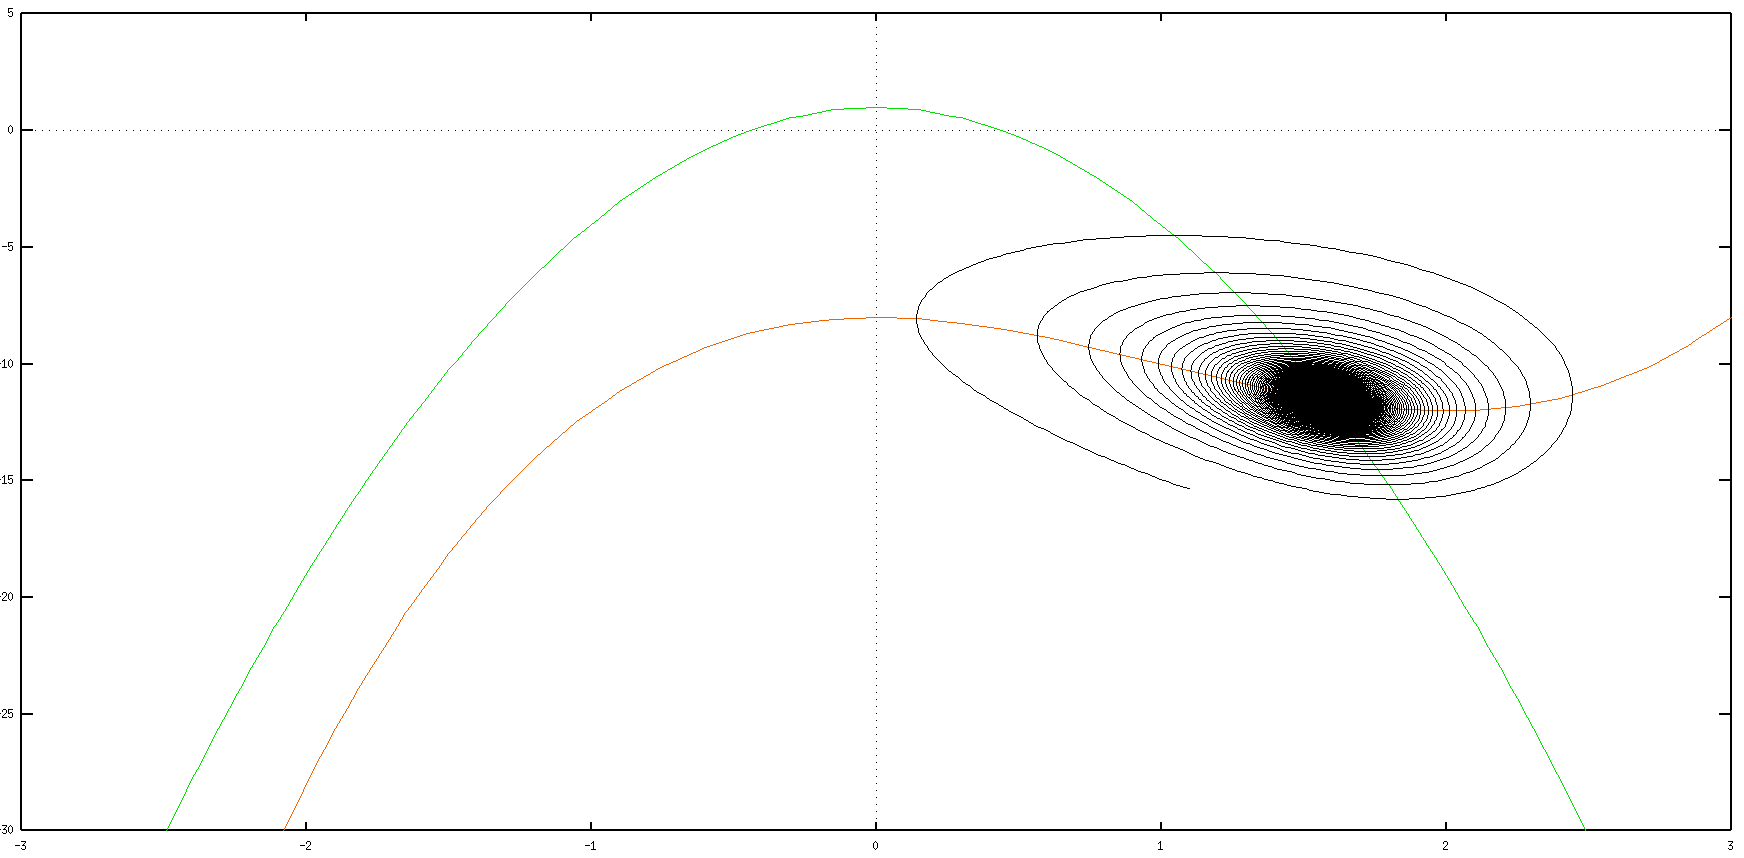
\includegraphics[height=5cm]{I_017}}
   \only<19> {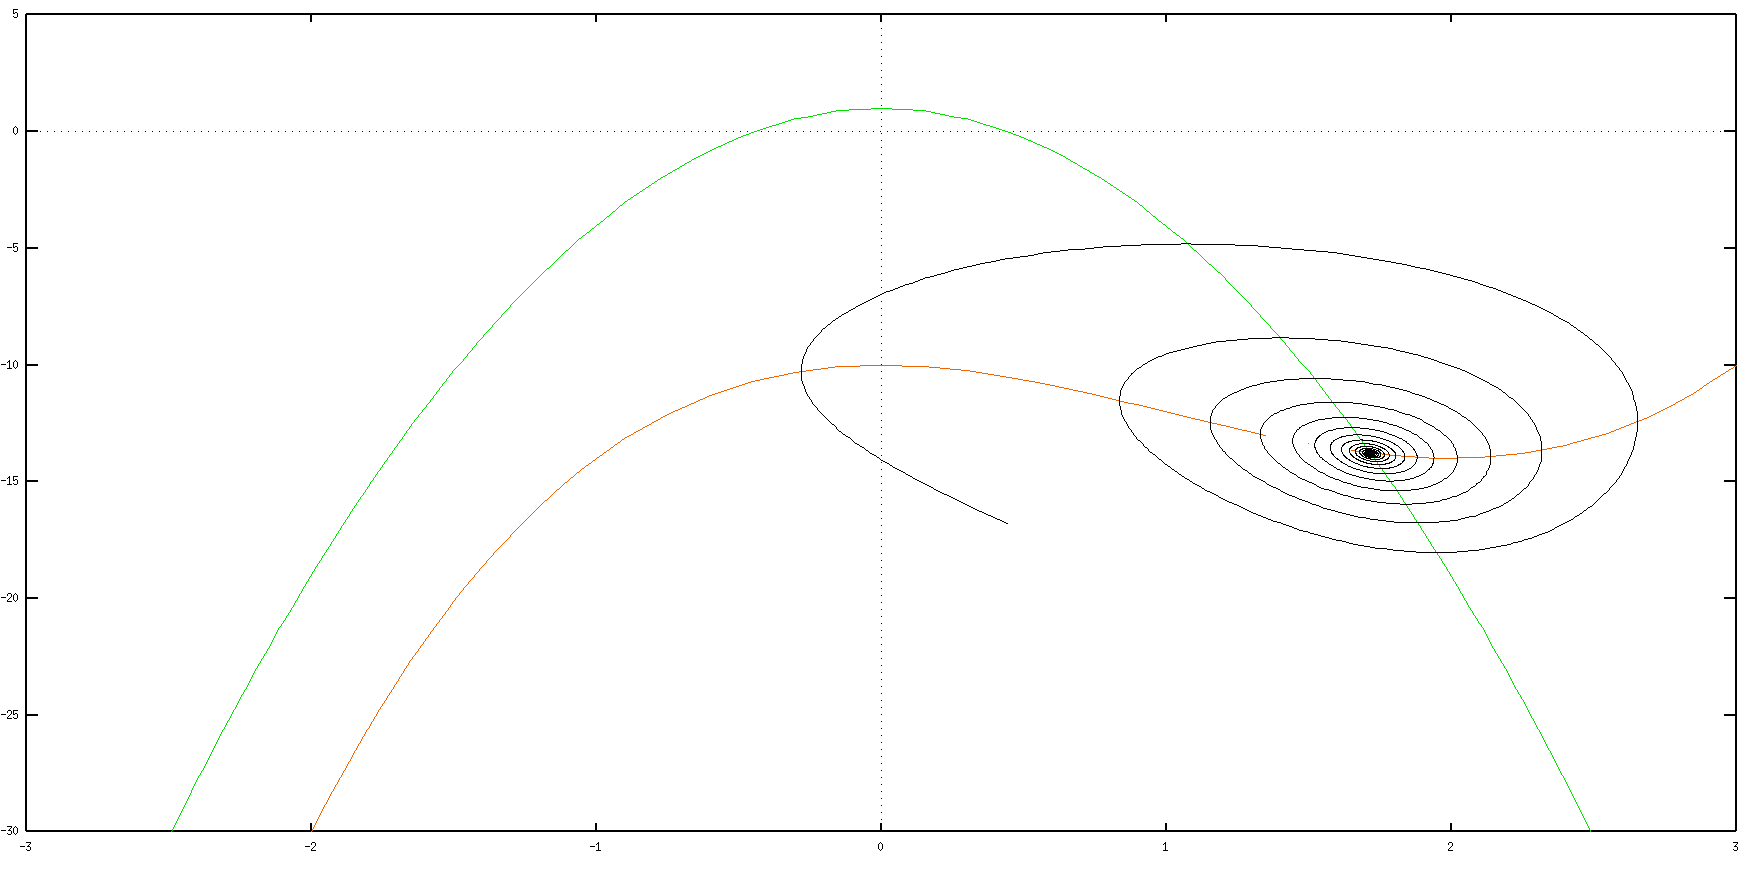
\includegraphics[height=5cm]{I_018}}


\end{frame}


\begin{frame}
\begin{center}
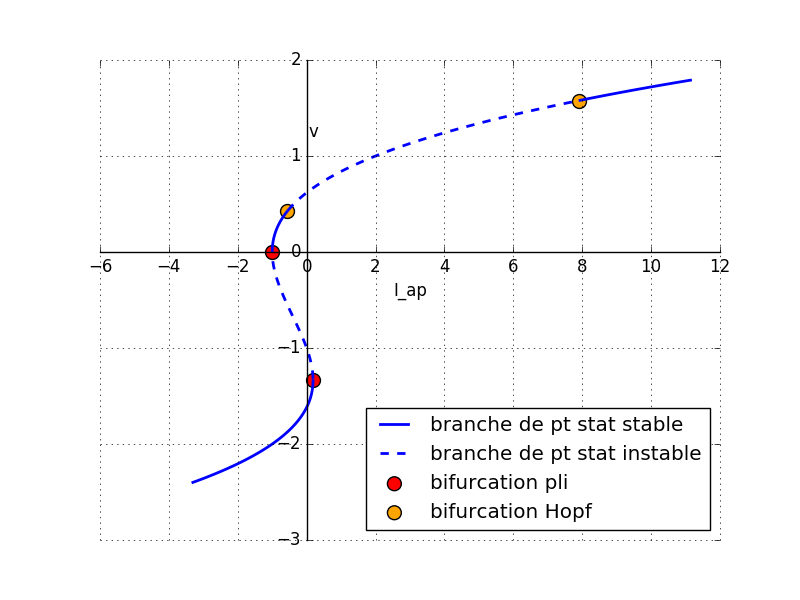
\includegraphics[width=0.6\textwidth]{bif4.png}
\end{center}
\end{frame}

\begin{frame}
\begin{small}
\begin{tabular}{|L{3.1cm} | C{0.5cm} | R{6cm}  |}
\hline
Valeur de $I_{ap}$ & N & Caractérisation des points \\
\hline
$I_{ap} \in [-2, -1[$ & 1 & noeud stable \\
\multicolumn{3}{|c|}{\textcolor{red}{\textbf{Bifurcation pli}}} \\
$I_{ap} = -1 $ & 2 & noeud stable et \textbf{col-noeud} \\\hline
$I_{ap} \in [-1, -0.988[$ & 3 & noeud stable, \textbf{col et noeud stable} \\\hline
$I_{ap} \in [-0.988, -0.567[$ & 3 & noeud stable, col et \textbf{foyer stable} \\
\multicolumn{3}{|c|}{\textcolor{Orange}{\textbf{Bifurcation Hopf}}} \\
$I_{ap} \in [-0.567, 5/27[$ & 3 & noeud stable, col, \textbf{foyer instable et cycle limite} \\\hline
$I_{ap} = 5/27 $ & 2 & \textbf{col-noeud}, foyer instable et cycle limite\\
\multicolumn{3}{|c|}{\textcolor{red}{\textbf{Bifurcation pli}}} \\
$I_{ap} \in [5/27, 7.90[$ & 1 &  foyer instable et cycle limite \\
\multicolumn{3}{|c|}{\textcolor{Orange}{\textbf{Bifurcation Hopf}}} \\
$I_{ap} \in [7.90, 10[$ & 1 &   foyer stable \\
\hline
\end{tabular}
\end{small}
\end{frame}


%----------------------SECTION 2---------------------------
%----------------------SECTION 2---------------------------
%----------------------SECTION 2---------------------------
%----------------------SECTION 2---------------------------


\section{Pour \texorpdfstring{$C=1$}{Lg}}
\begin{frame}
\tableofcontents[currentsection]
\end{frame}


\begin{frame}{Diagramme de bifurcation}
\begin{figure}[H]
    \begin{center}
    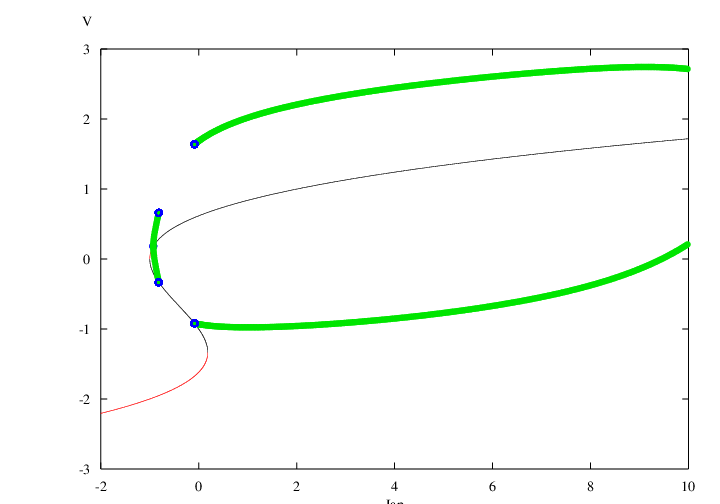
\includegraphics[width=5.5cm]{Diag_bif_c_1.png}
    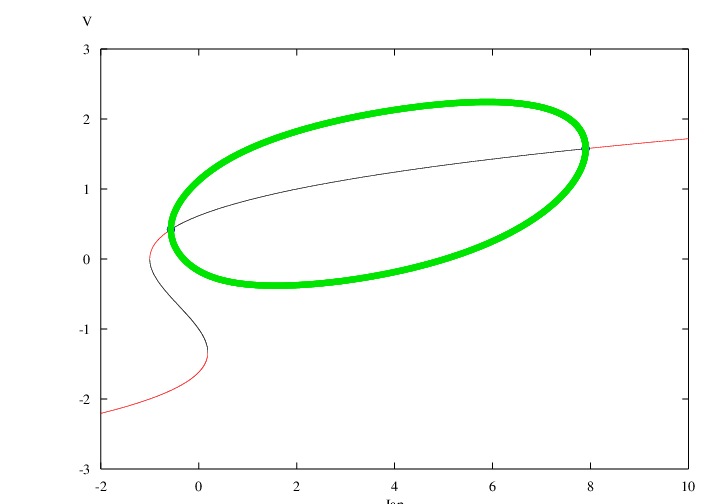
\includegraphics[width=5.5cm]{Diag_bif_c_2.png}
    \caption{Diagramme de bifurcation pour $c = 1$ (à gauche) et $c = 2$ (à droite)}
    \end{center}
\end{figure}

\end{frame}

\begin{frame}{Stabilité et bifurcation}
\begin{itemize}
\item Mêmes branches de points stationnaires, stabilité qui varie avec c :
\begin{itemize}
\item Les points de bifurcations de Hopf s'éloignent
\item La famille de cycle limite rencontre la branche du col : \textbf{bifurcation homocline}
\end{itemize}
\item Bifurcations pli indépendantes de $c$.
\end{itemize}

\end{frame}


\begin{frame}
\only<1>{Pour $c=1$ et $I_{ap}=-2.0$ \\ 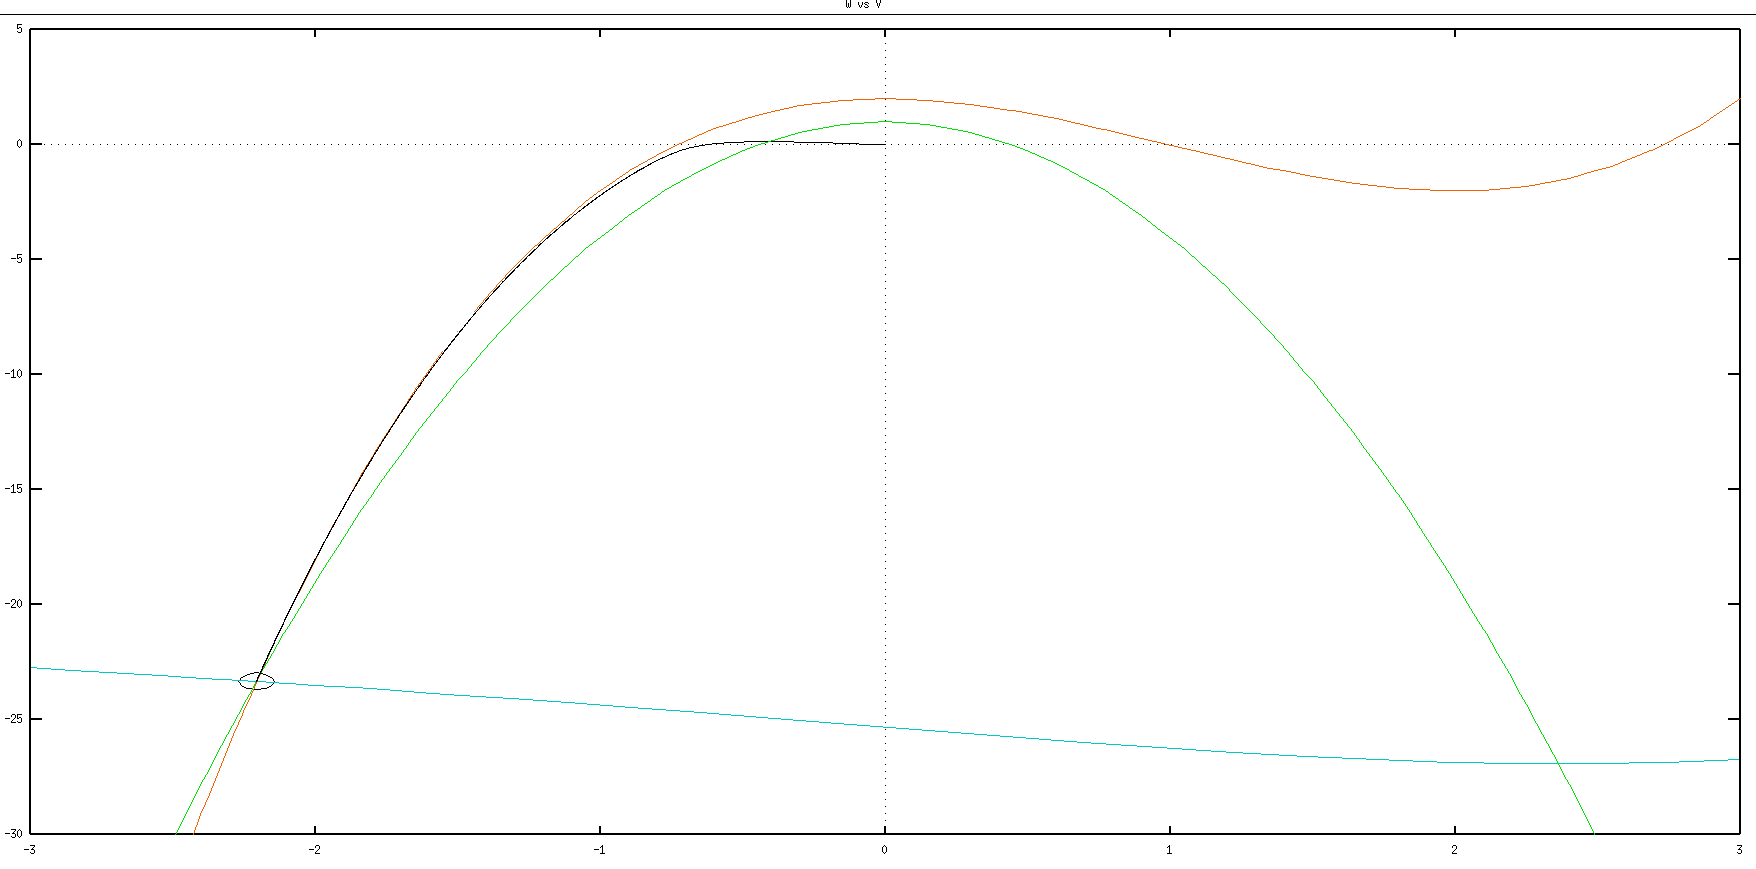
\includegraphics[height=5cm]{1I-2.png}}

\only<2>{Pour $c=1$ et $I_{ap}=-1.15$ \\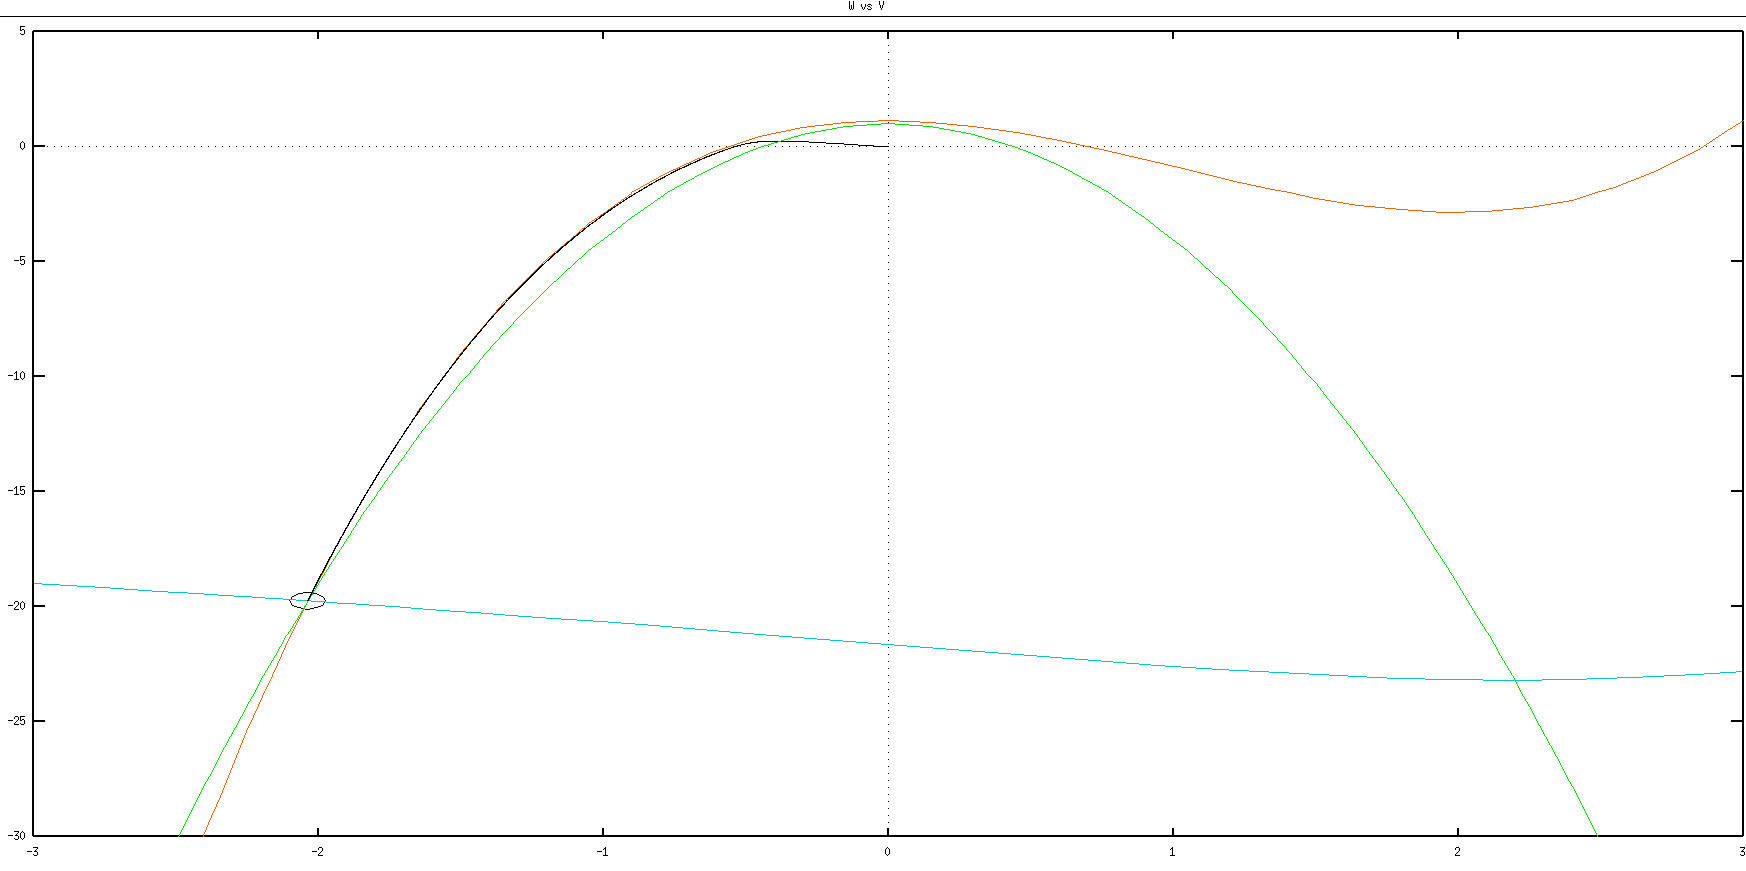
\includegraphics[height=5cm]{3I-1_15.png}}

\only<3>{Pour $c=1$ et $I_{ap}=-1.0$ \\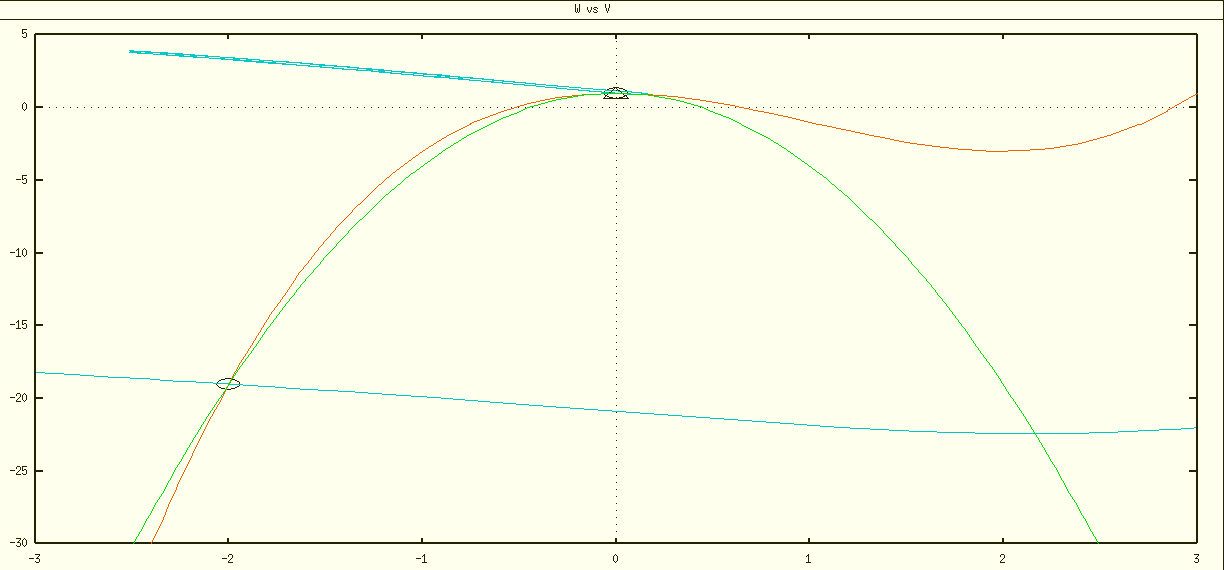
\includegraphics[height=5cm]{I-1.png}}
\only<4>{Pour $c=1$ et $I_{ap}=-1.0$ \\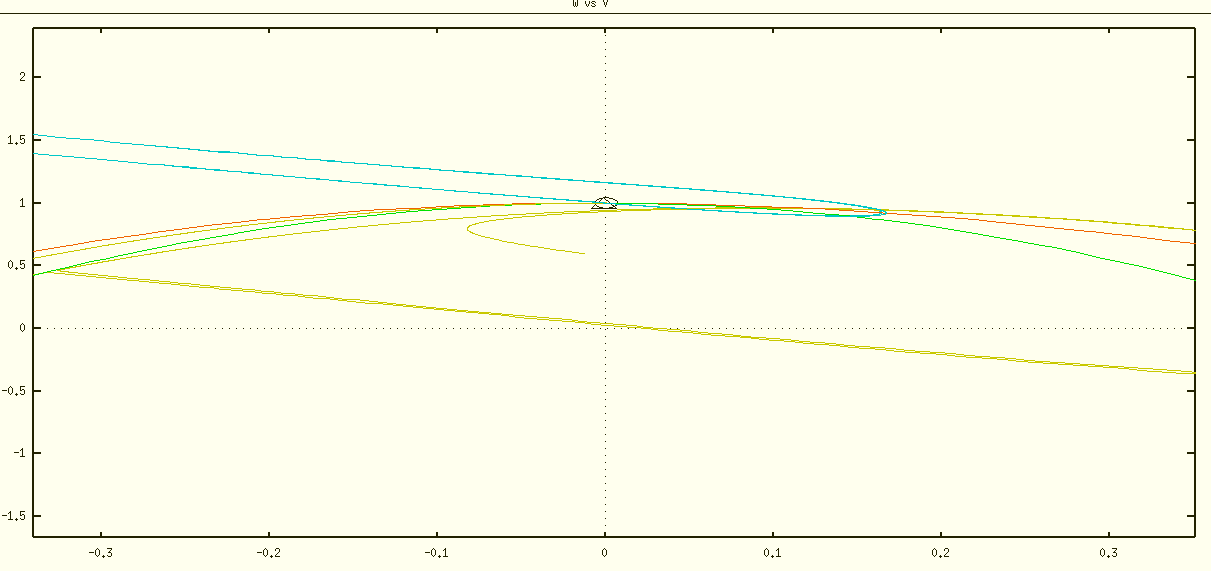
\includegraphics[height=5cm]{I-1Bis.png}}
\only<5>{Pour $c=1$ et $I_{ap}=-1.0$ : deux bassins d'attraction séparés par variété stable
\\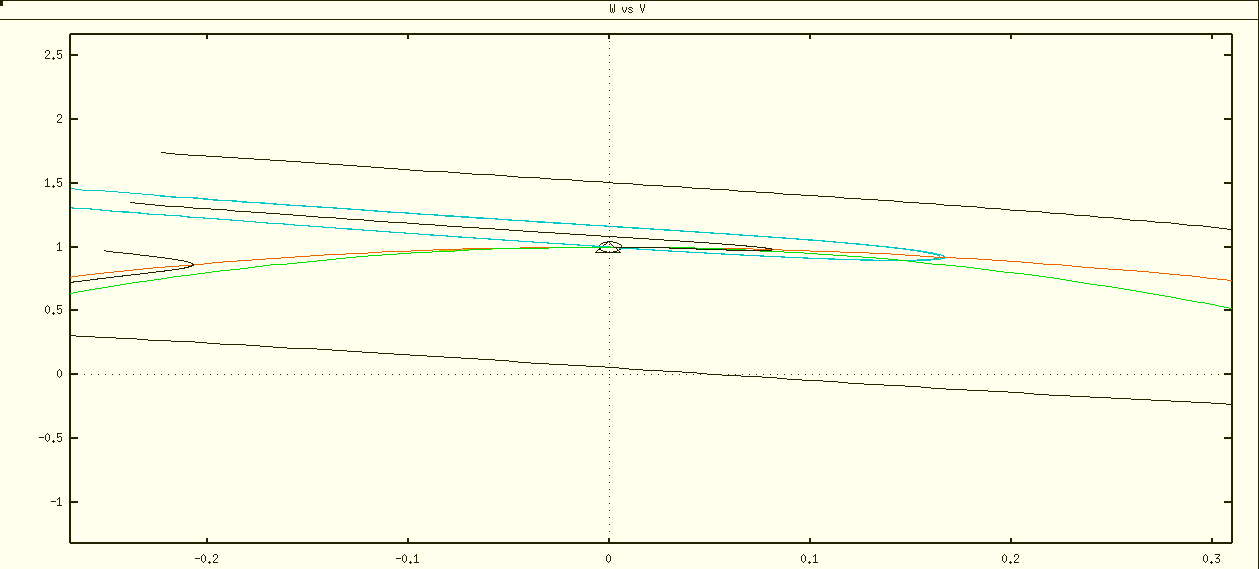
\includegraphics[height=5cm]{I-1Ter.png}}

\only<6>{Pour $c=1$ et $I=-0.997$ \\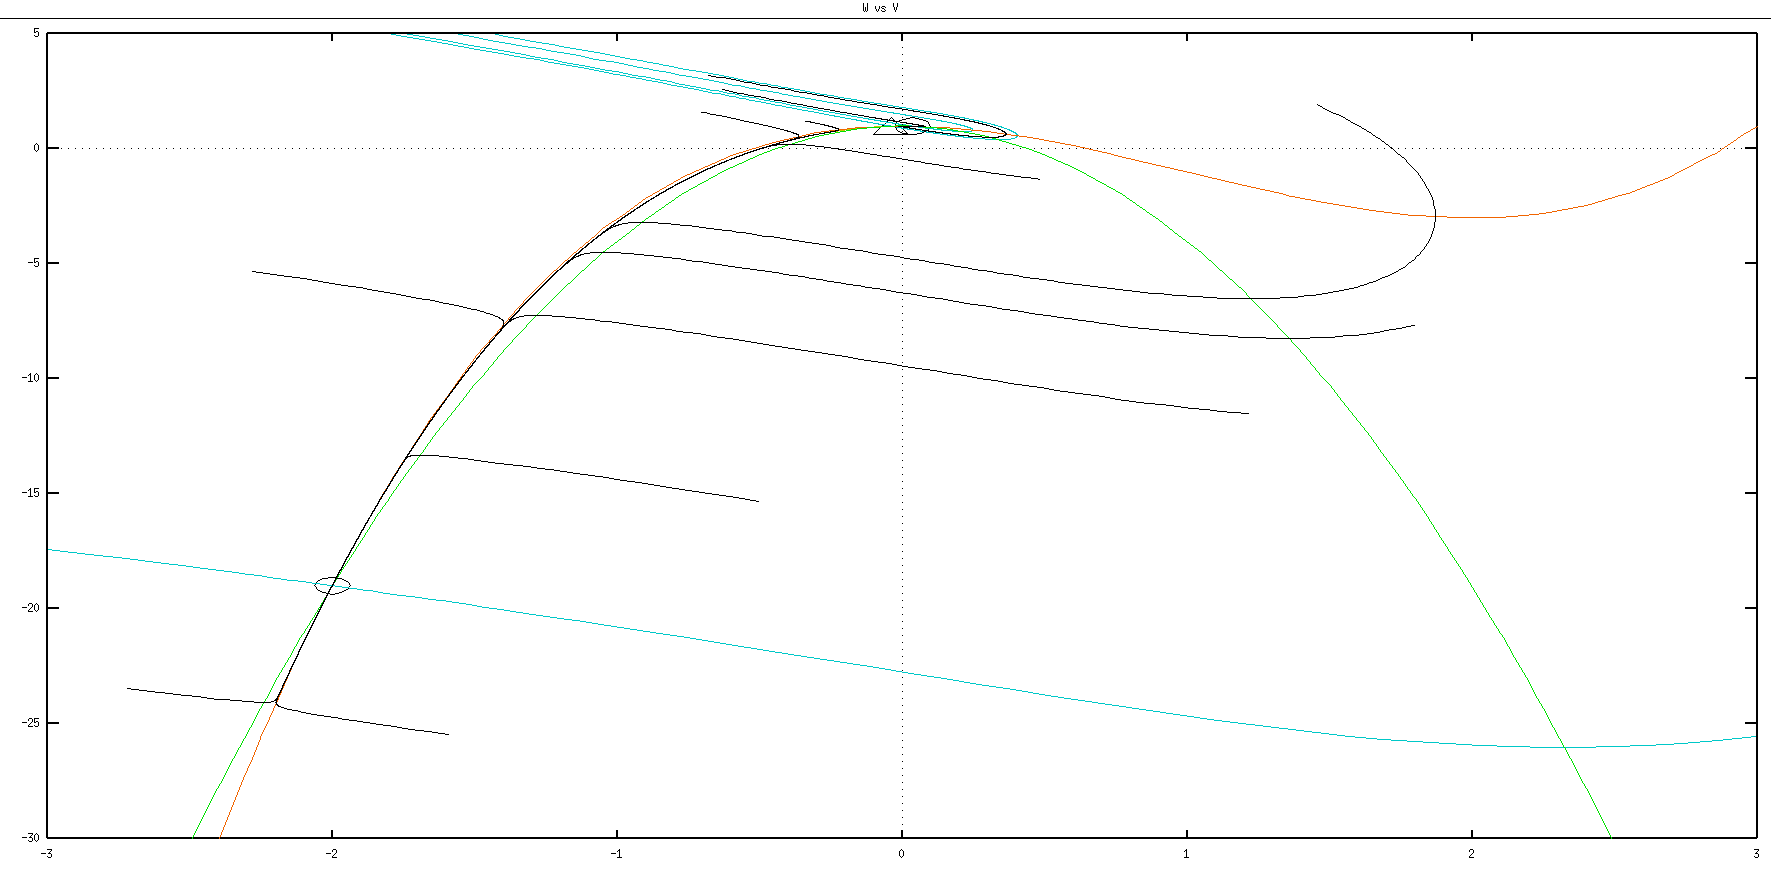
\includegraphics[height=5cm]{6I-0_9971.png}}
\only<7>{Pour $c=1$ et $I=-0.997$ \\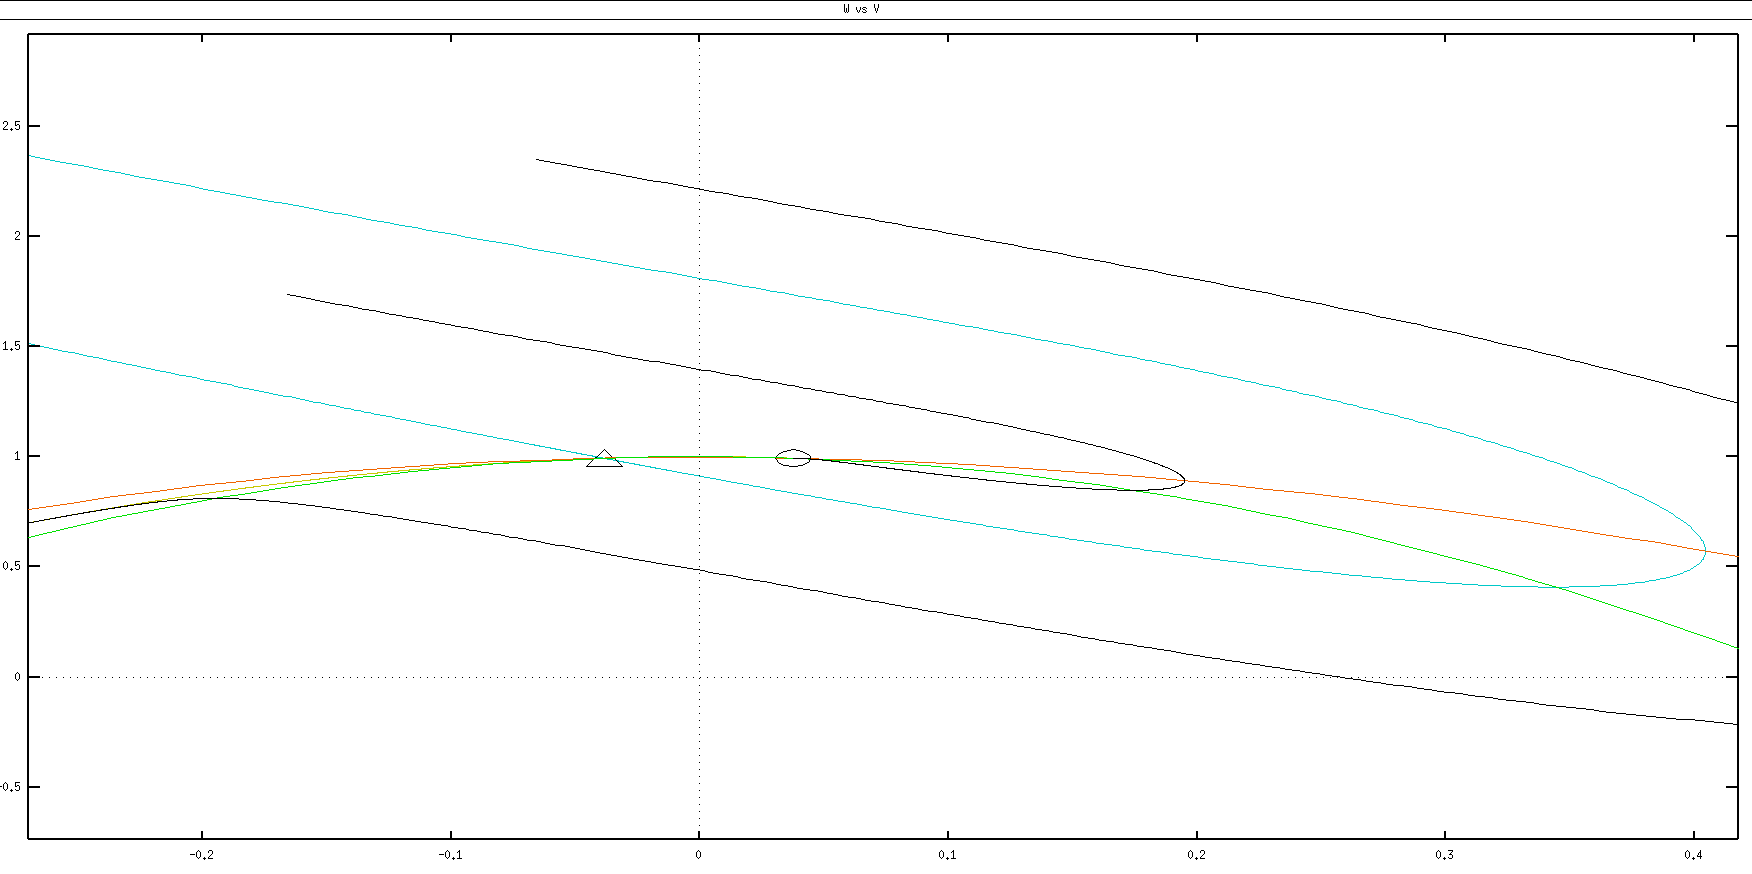
\includegraphics[height=5cm]{6I-0_9971Bis.png}}

\only<8>{Pour $c=1$ et $I_{ap}=-0.94$ \\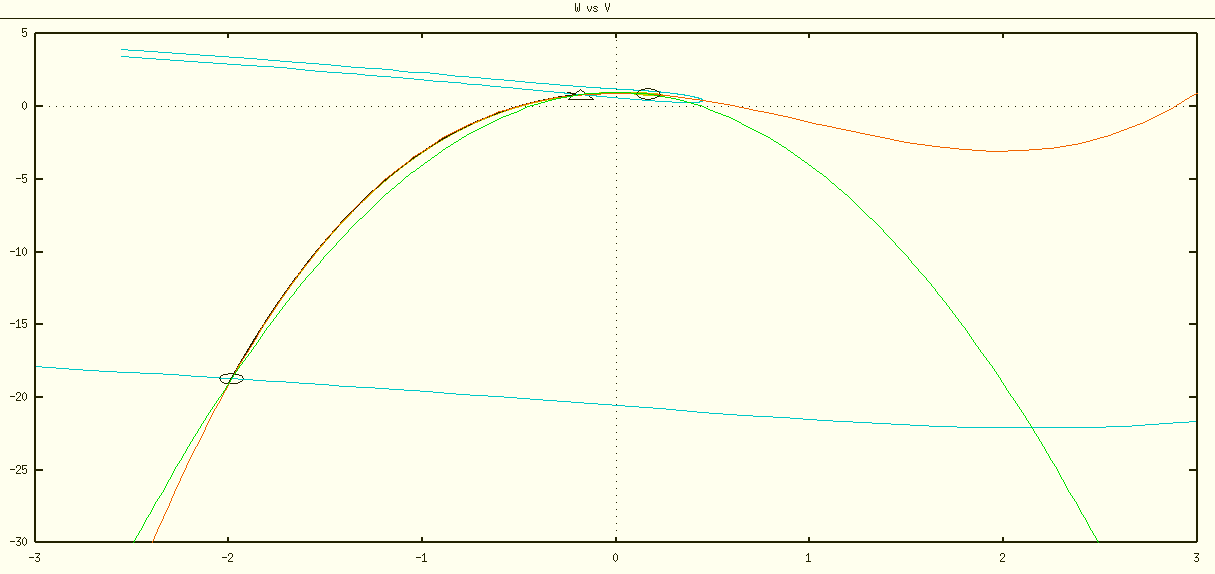
\includegraphics[height=5cm]{I-0_94.png}}
\only<9>{Pour $c=1$ et $I_{ap}=-0.94$ \\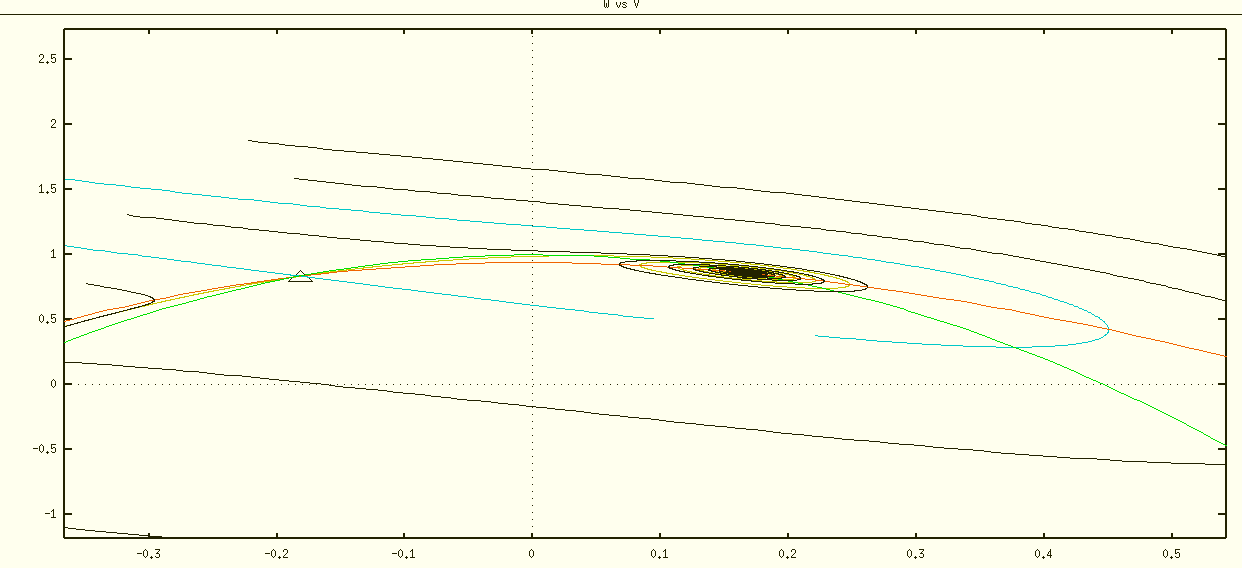
\includegraphics[height=5cm]{I-0_94Bis.png}}


\only<10>{Pour $c=1$ et $I=-0.82$ \\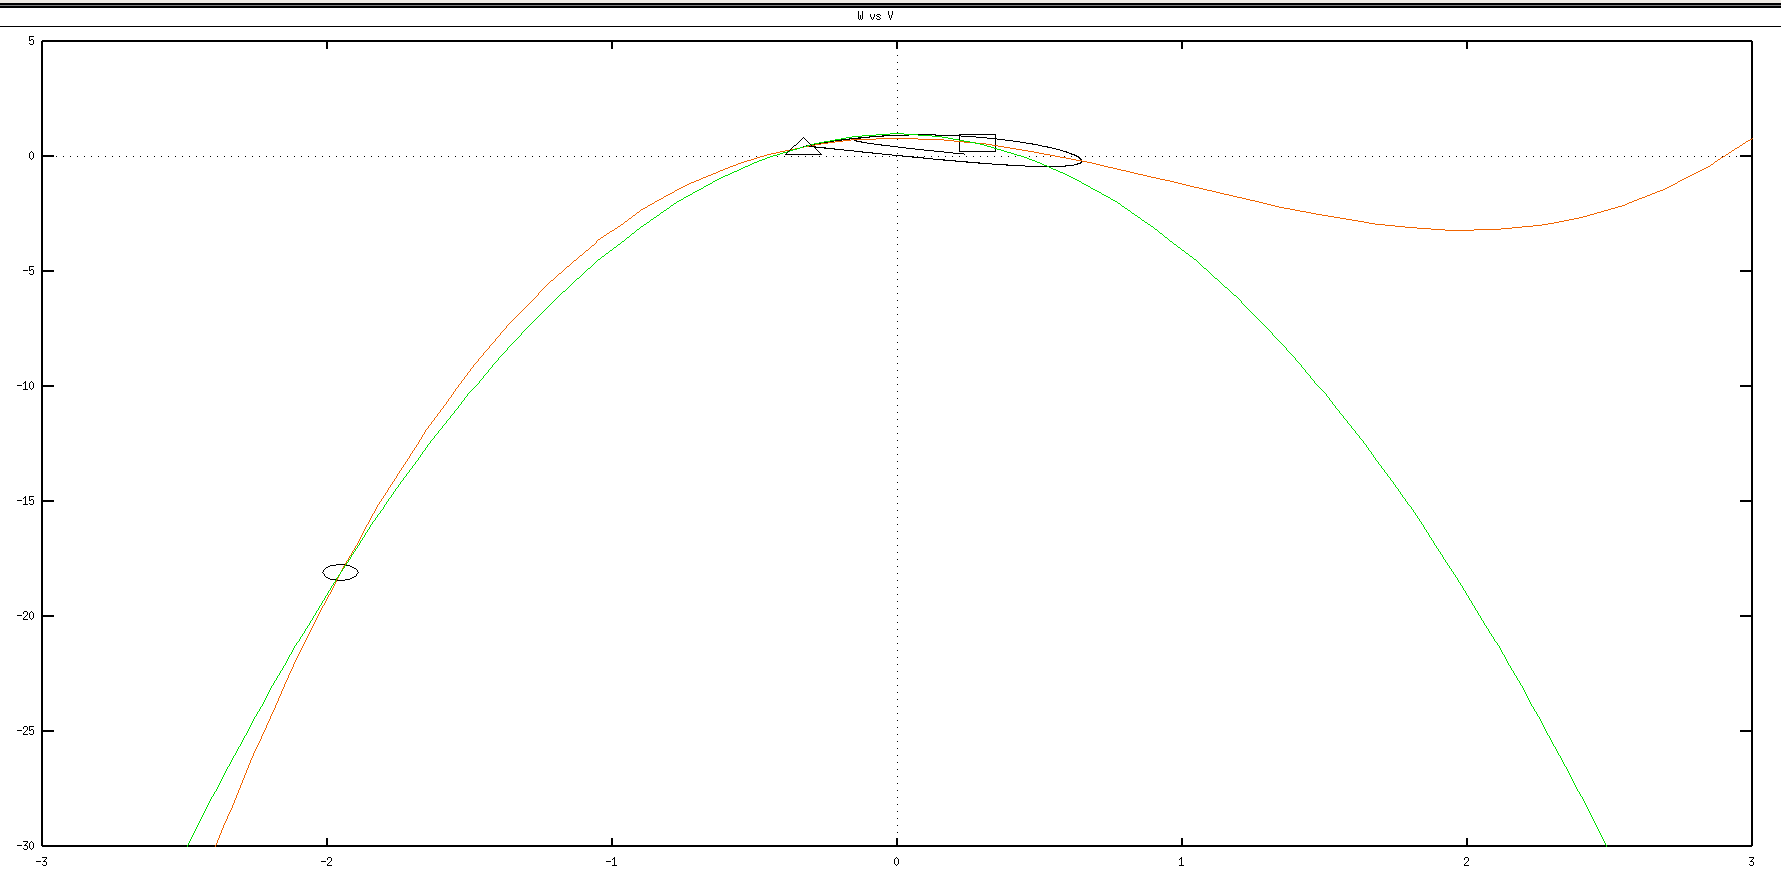
\includegraphics[height=5cm]{8I-0_82.png}}

\only<11>{Pour $c=1$ et $I=-0.816$ \\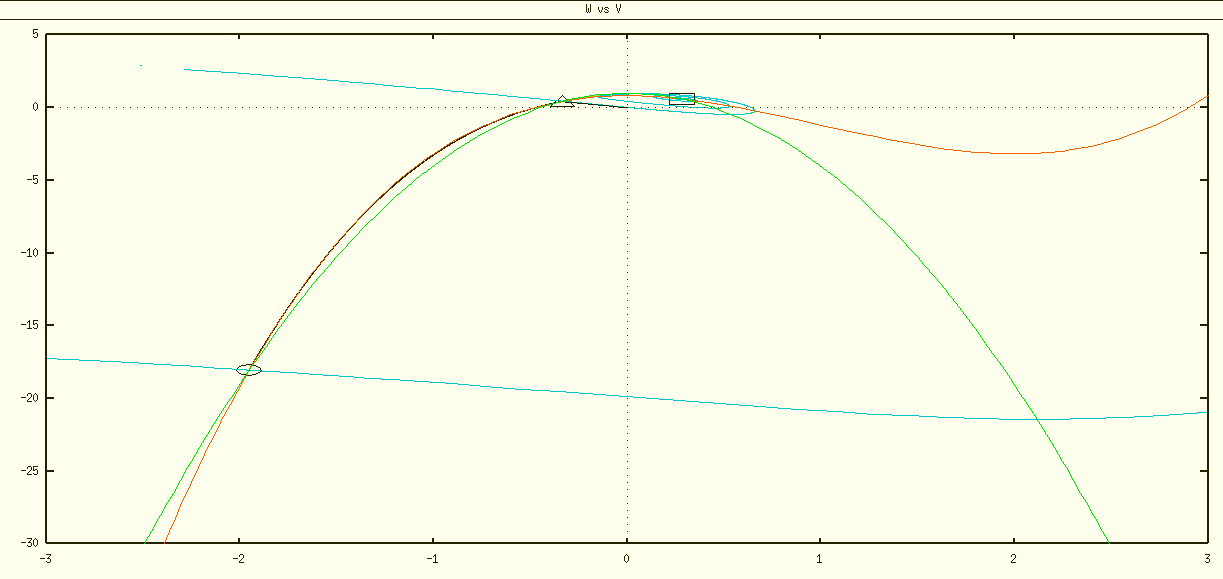
\includegraphics[height=5cm]{I-0_816.png}}
\only<12>{Pour $c=1$ et $I=-0.816$ \\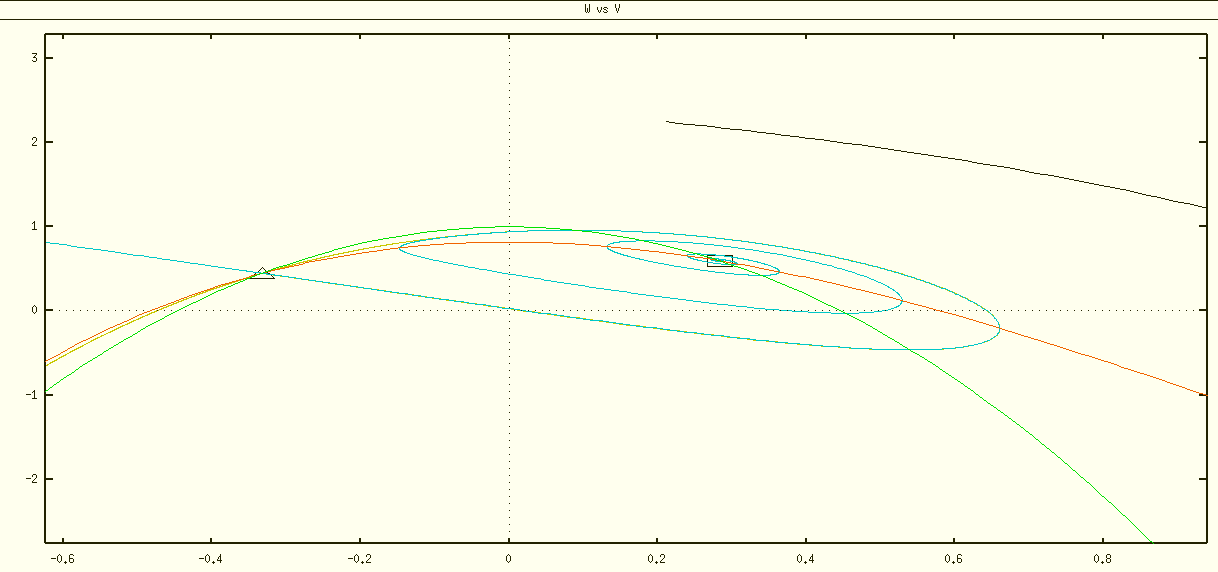
\includegraphics[height=3.5cm]{I-0_816Bis.png}
\\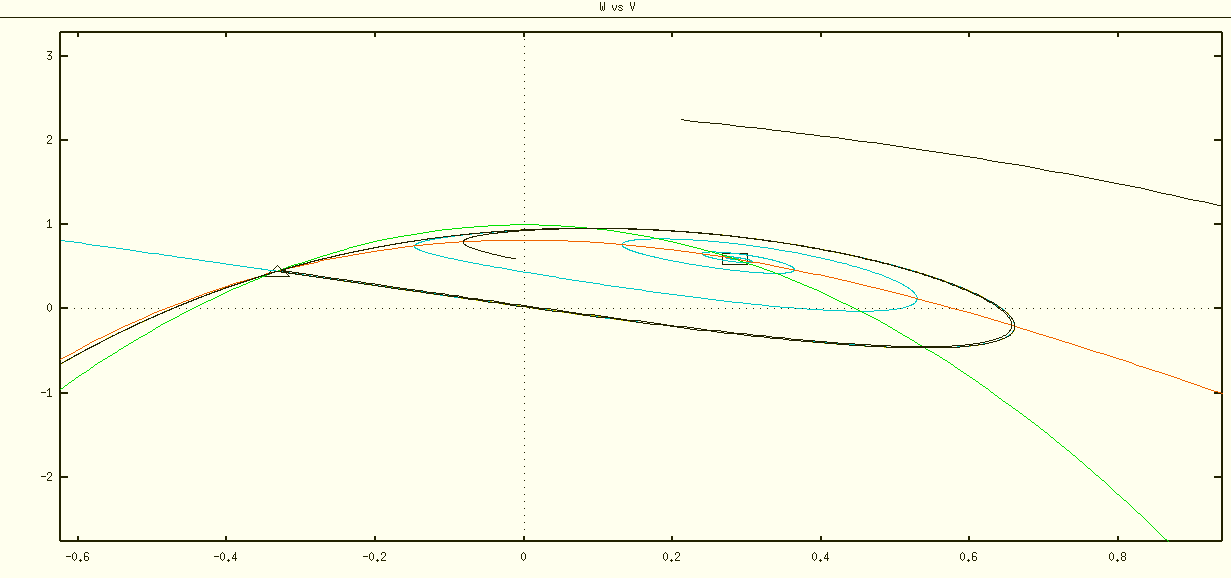
\includegraphics[height=3.5cm]{I-0_816Ter.png}}

\only<13>{Pour $c=1$ et $I=-0.816$ \\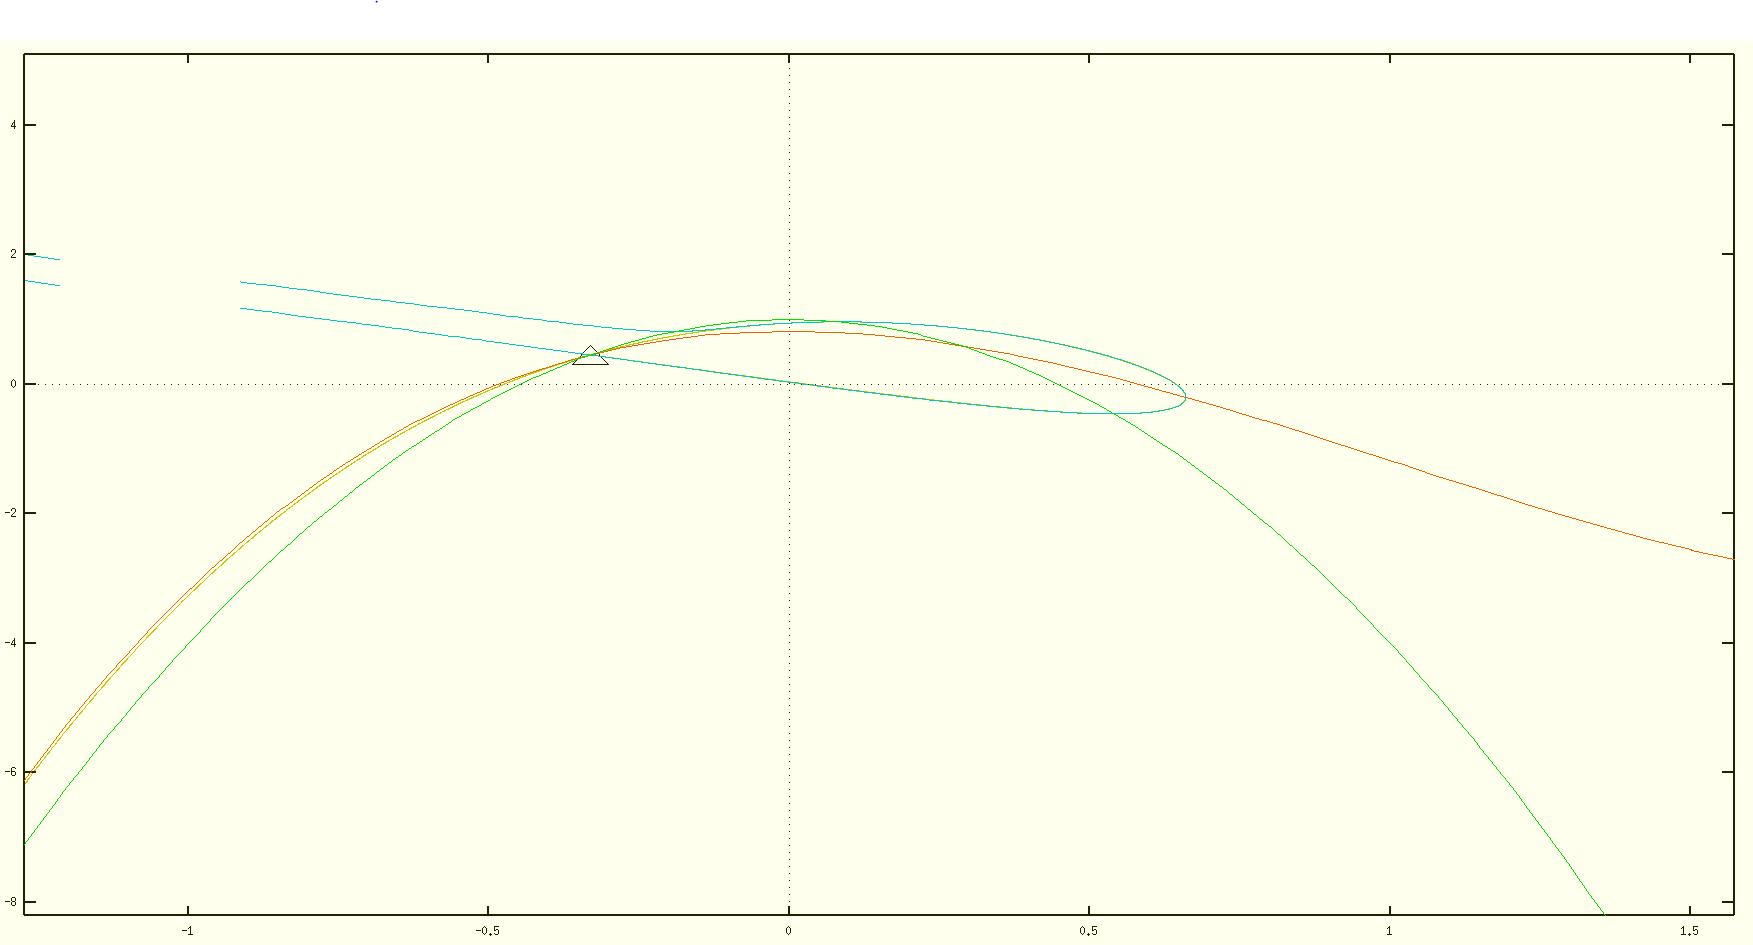
\includegraphics[height=5cm]{I-0_816Qua.png}}

\only<14>{Pour $c=1$ et $I=-0.5$ \\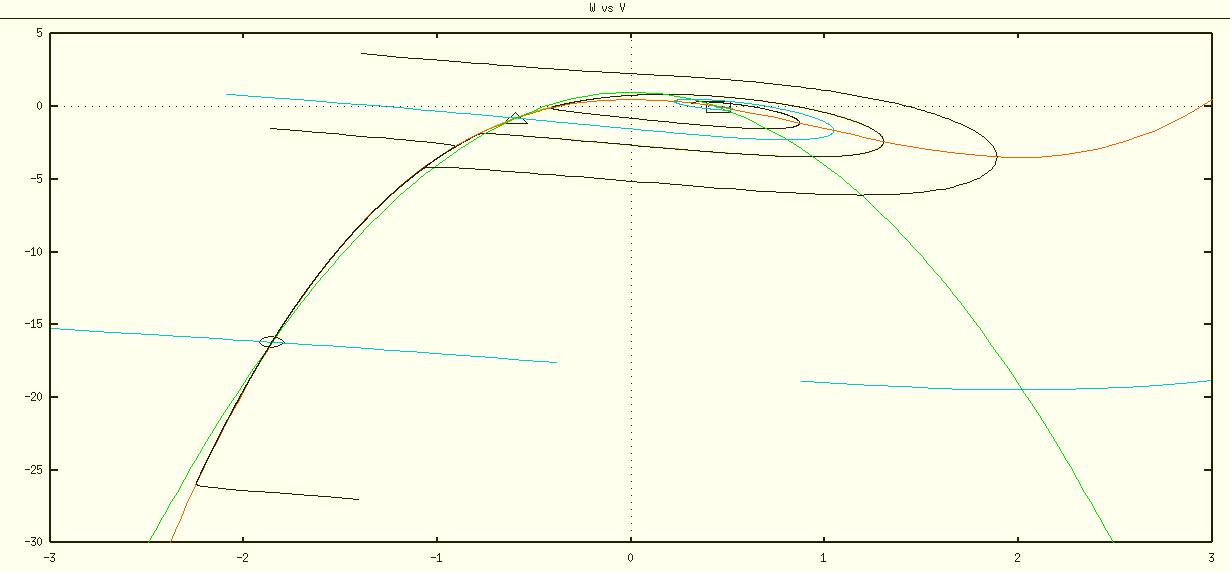
\includegraphics[height=5cm]{I-0_5.png}}

\only<15>{Pour $c=1$ et $I=-0.08$ \\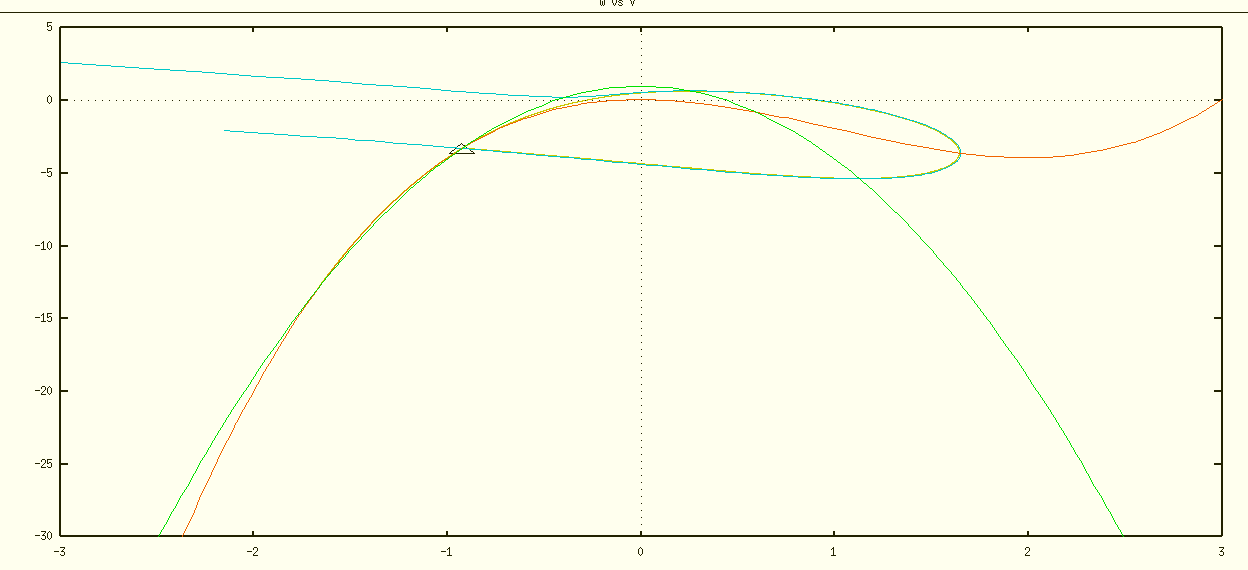
\includegraphics[height=5cm]{I-0_08.png}}


\only<16>{Pour $c=1$ et $I=0.0$ \\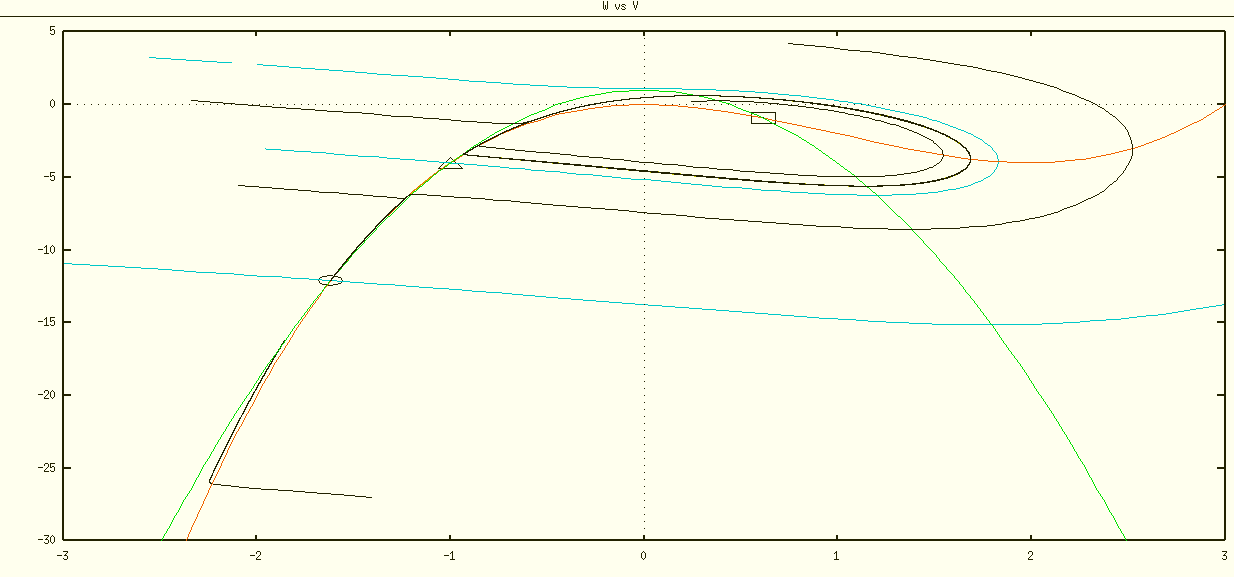
\includegraphics[height=5cm]{I0.png}}

\only<17>{Pour $c=1$ et $I=0.18$ \\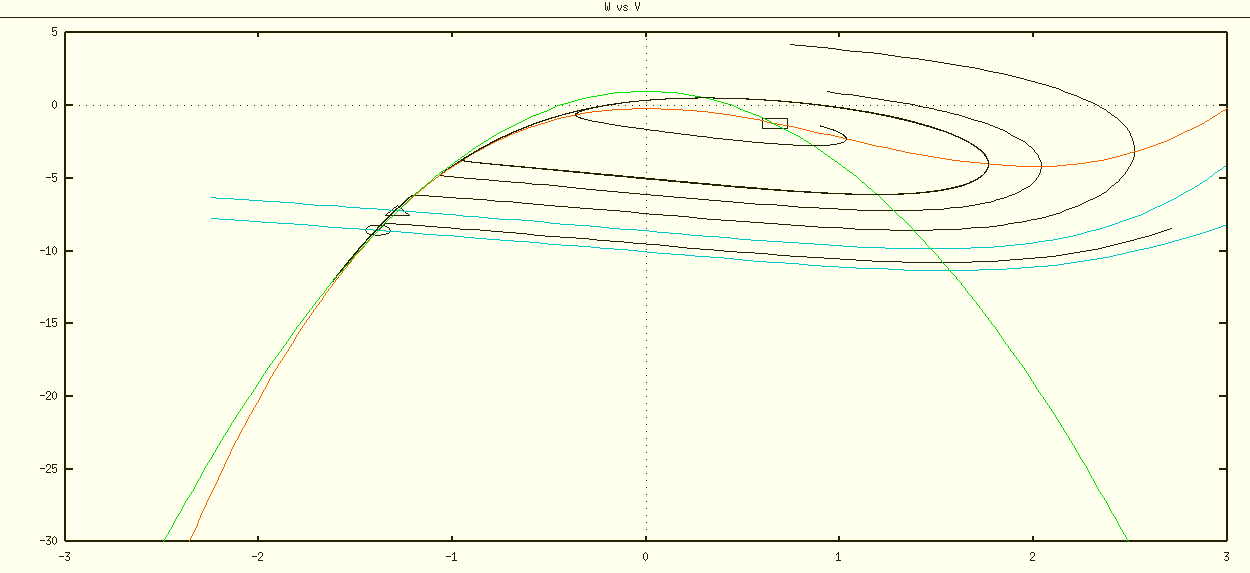
\includegraphics[height=5cm]{I0_18.png}}
\only<18>{Pour $c=1$ et $I=0.185$ \\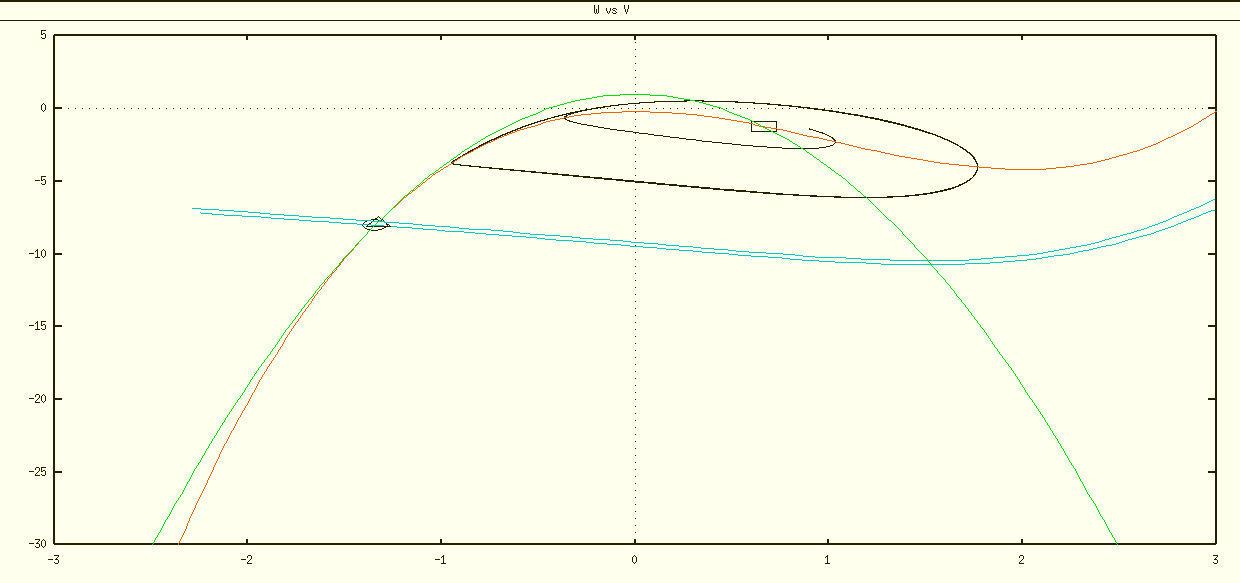
\includegraphics[height=5cm]{I0_185.png}}

\only<19>{Pour $c=1$ et $I=0.5$ \\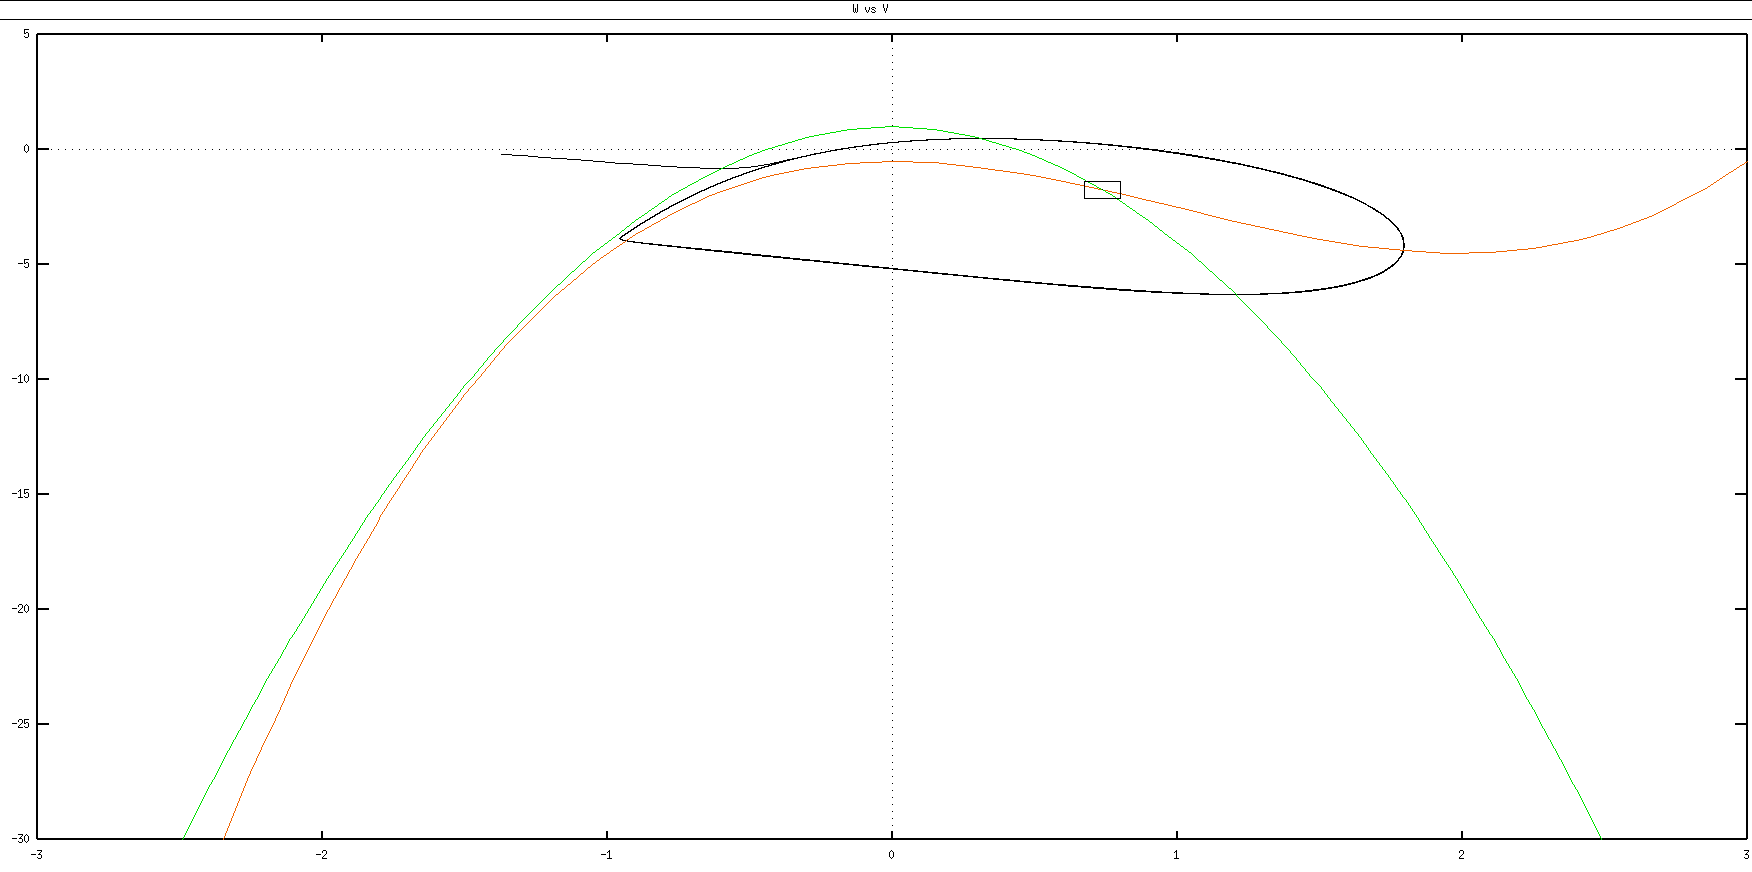
\includegraphics[height=5cm]{14I0_5.png}}
\only<20>{Pour $c=1$ et $I=1.5$ \\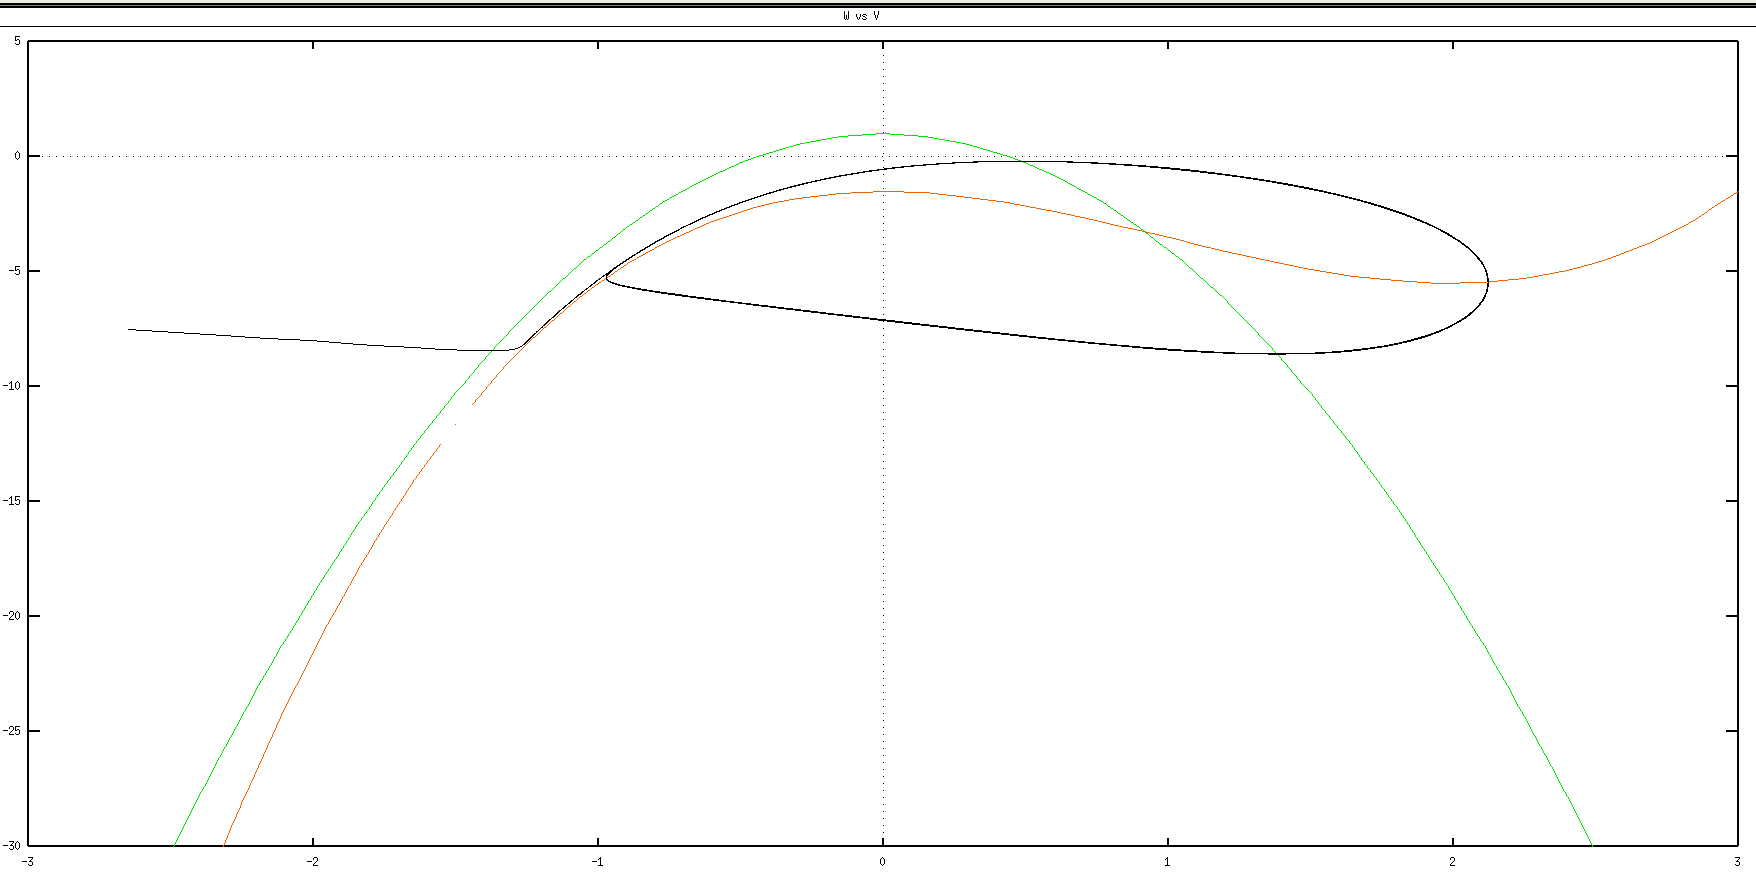
\includegraphics[height=5cm]{15I1_5.png}}
\only<21>{Pour $c=1$ et $I=2.0$ \\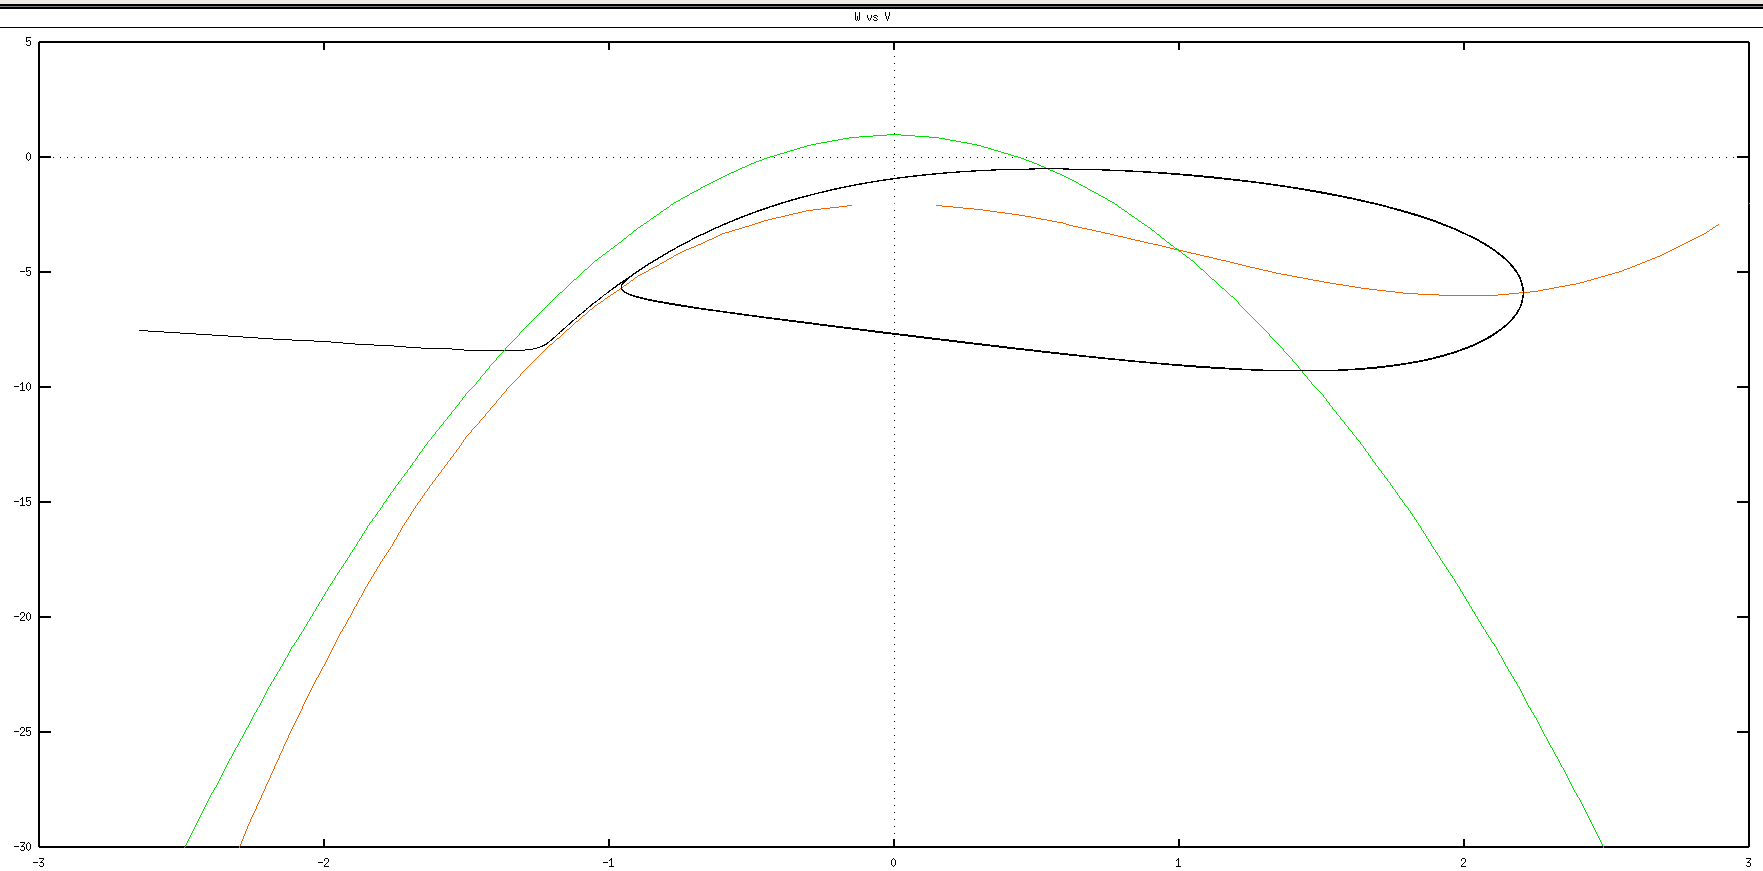
\includegraphics[height=5cm]{16I2.png}}

\only<22>{Pour $c=1$ et $I=5.5$ \\\includegraphics[height=5cm]{18I5_5.png}}
\only<23>{Pour $c=1$ et $I=10.0$ \\\includegraphics[height=5cm]{19I10.png}}

\end{frame}

\begin{frame}{Récapitulatif}
\begin{small}
\begin{tabular}{|L{3.3cm} | C{0.5cm} | R{6.5cm}  |}
\hline
Valeur de $I_{ap}$ & N & \textbf{Caractérisation des points} \\
\hline
$I_{ap} \in ]-2, -1[$ & 1 & noeud stable \\
\multicolumn{3}{|c|}{\textcolor{red}{\textbf{Bifurcation pli}}} \\
$I_{ap} = -1 $ & 2 & noeud stable et \textbf{col-noeud} \\\hline
$I_{ap} \in ]-1, -0.9971[$ & 3 & noeud stable et \textbf{col et noeud stable} \\\hline
$I_{ap} \in ]-0.9971, -0.926[$ & 3 & noeud stable, col et \textbf{foyer stable} \\
\multicolumn{3}{|c|}{\textcolor{Orange}{\textbf{Bifurcation Hopf}}} \\
$I_{ap} \in ]-0.926, -0.816[$ & 3 & noeud stable, col et \textbf{foyer instable, cycle limite} \\\hline
\multicolumn{3}{|c|}{\textcolor{NavyBlue}{\textbf{Bifurcation homocline}}} \\
$I_{ap} \in ]-0.816, -0.0856[$ & 3 & noeud stable, col et \textbf{foyer instable} \\\hline
\multicolumn{3}{|c|}{\textcolor{NavyBlue}{\textbf{Bifurcation homocline}}} \\
$I_{ap} \in ]-0.0856, 5/27[$ & 3 & noeud stable, col, foyer instable, \textbf{cycle limite} \\\hline
$I_{ap} = 5/27 $ & 2 & \textbf{col-noeud}, foyer instable et cycle limite\\
\multicolumn{3}{|c|}{\textcolor{red}{\textbf{Bifurcation pli}}} \\
$I_{ap} \in ]5/27, 10[$ & 1 &  foyer instable et cycle limite \\
\hline
\end{tabular}
\end{small}

\end{frame}


%----------------------SECTION 3---------------------------
%----------------------SECTION 3---------------------------
%----------------------SECTION 3---------------------------
%----------------------SECTION 3---------------------------

\section{Passage en 3 dimensions : bursting}

\begin{frame}
\tableofcontents[currentsection]
\end{frame}

\begin{frame}{Nouveau système}

\begin{equation}
\left\{
\begin{array}{l }
v'(t)= (w - v^3 + 3v^2 +I_{ap})/c = f(v,w) \\
w'(t) = 1 - 5 v^2 - w = g(v,w)  \\
\textcolor{Blue}{I_{ap}'(t)= \varepsilon (0.3 I_{ap} -1 -v)}
\end{array}
\right.
\end{equation}

\begin{itemize}
\item pour $c=2$ et $c=1$ : existence de zones de \textbf{multistabilité} dans le sous système rapide $(v,w)$
\item $I'_{ap} = \epsilon(0.9v^3+0.6v^2-v-1.3)$ si $v = v_0$
\item racines de $I'_{ap} = 0$ :
\end{itemize}
\begin{center}
$\left\{
\begin{array}{rl}
v_1 &\approx -2.64087\\
v_2 &\approx -1\\
v_3 &\approx 1.64087\\
\end{array}
\right.$

\end{center}
\end{frame}

\subsection{Obtention du bursting}


\begin{frame}{Hystérèse}
\begin{center}
\begin{tiny}
\begin{tabular}{|L{1cm} | C{0.8cm} | C{0.8cm} | C{0.8cm} |C{0.8cm}|C{0.8cm}|C{0.8cm}|C{0.8cm}|}
\hline
\multicolumn{8}{|c|}{$c \in [1, 2]$}
\\\hline
Valeur de $v$ & $v < -2.64$ & $v = -2.64$ & $ -2.64 < v < -1$ & $v = -1$ & $-1 < v < 1.64$ & $v=1.64$ & $v > 1.64$ \\
 \hline
$I'_{ap}$ & - & 0 & + & 0 & - & 0 & +\\ \hline
\end{tabular}
\end{tiny}
\includegraphics[height = 7cm, angle = 270]{Diag_bif_c_2.eps}
\end{center}
\end{frame}

\begin{frame}{Superposition de la trace en temps de $I_{ap}$}
\begin{center}
\only<1>{$c = 1$ \\ \includegraphics[height = 8cm, angle=270, origin =c]{Iap_c_1.png}}
\only<2>{$c = 2$ \\\includegraphics[height = 8cm, angle=270, origin =c]{Iap_c_2.png}}
\only<3>{pour $c=2$ et $c=1$ \\\includegraphics[height = 6cm, origin = c]{superpose_Iap.png}}
\end{center}
\end{frame}

\begin{frame}{Récapitulatif}
Contexte :
\begin{itemize}
\item $I_{ap}$ variable lente ($\epsilon$ aussi petit que l'on veut), $(v, w)$ variables rapides
\item Sous système rapide bistable pour $c \in [1 ; 2]$
\begin{itemize}
\item branche de noeuds
\item famille de cycles limites
\end{itemize}
\item Phénomène d'hystérèse
\end{itemize}
Observations :
\begin{itemize}
\item Amplitude de $I_{ap}$ 4 fois plus importante pour $c = 2$
\item Fréquence 2 fois plus élevée pour $c = 1$
\end{itemize}
\end{frame}

\subsection{Pour \texorpdfstring{$c = 2$}{Lg} : Bursting fold/Hopf}

\subsubsection*{Bursting \texorpdfstring{$V=f(t)$}{Lg}}

\begin{frame}{Bursting temporel $v=f(t)$ pour $c = 2$}
\begin{center}
\href{https://drive.google.com/open?id=0ByPBcq8q0ou_c0xJOVRmR2JHd2M}{\includegraphics[width =  1.0\textwidth]{Burst_c_2_temp}}
\end{center}
\end{frame}

\subsubsection*{Bursting dans le plan de phase \texorpdfstring{$W=f(V)$}{Lg}}


\begin{frame}{Bursting dans le plan de phase $v=f(t)$ pour $c = 2$}
\begin{center}
\href{https://drive.google.com/open?id=0ByPBcq8q0ou_TFloLXphQjVBQ0k}{\includegraphics[width =  1.0\textwidth]{Burst_c_2_phase}}
\end{center}
\end{frame}

\subsubsection*{Superposition diagramme de bifurcation du sous-système rapide et \texorpdfstring{$v=f(I_{ap})$}{Lg}}


\begin{frame}{Superposition diagramme de bifurcation du sous-système rapide et $v=f(I_{ap})$}
\begin{center}
\includegraphics[height = 7cm]{superpositionC2}
\end{center}
\end{frame}

\begin{frame}{Récap bursting pour c=2}
\begin{center}
\begin{itemize}
\item Début du burst par bifurcation pli
\item Fin du burst par bifurcation de Hopf surcritique
\item Amplitude des spikes décroissante
\item Fréquence des spikes constante $\approx 2\pi$
\item $v_{rest} \ne v_{burst}$
\end{itemize}
\vspace{1cm}
Classification de Izhikevich : \textbf{fold/Hopf}
\end{center}
\end{frame}

\subsection{Pour \texorpdfstring{$c = 1$}{Lg} : Bursting Square-Wave}

\subsubsection*{Bursting \texorpdfstring{$V=f(t)$}{Lg}}

\begin{frame}{Bursting temporel $v=f(t)$ pour $c = 1$}
\begin{center}
\href{https://drive.google.com/open?id=0ByPBcq8q0ou_cmtOazZJZFFIN2M}{\includegraphics[width =  1.0\textwidth]{Burst_c_1_temp}}
\end{center}
\end{frame}

\subsubsection*{Bursting dans le plan de phase \texorpdfstring{$W=f(V)$}{Lg}}

\begin{frame}{Bursting dans le plan de phase $v=f(t)$ pour $c = 1$}
\begin{center}
\href{https://drive.google.com/open?id=0ByPBcq8q0ou_SDgyV19GRTRiQ2M}{\includegraphics[width =  1.0\textwidth]{Burst_c_1_phase}}
\end{center}
\end{frame}

\subsubsection*{Superposition diagramme de bifurcation du sous-système rapide et \texorpdfstring{$V=f(I_{ap})$}{Lg}}


\begin{frame}
\begin{center}
\includegraphics[width = 1\textwidth]{superpositionC1}
\end{center}
\end{frame}

\begin{frame}{Récap bursting pour c=1}
\begin{center}
\begin{itemize}
\item Début du burst par bifurcation pli
\item<2,3,4,5> Fin du burst par bifurcation homocline
\item<3,4,5> Amplitude des spikes constante
\item<4,5> Fréquence décroissante et tend vers 0.
\item<5> $v_{rest} \ne v_{burst}$
\end{itemize}
\vspace{1cm}
Classification de Rinzel : \textbf{Square-Wave}
\end{center}
\end{frame}

\subsection{Entre \texorpdfstring{$c = 1$}{Lg} et \texorpdfstring{$c = 2$}{Lg}}

\subsubsection*{Trace en temps et fréquence des spikes en fonction de c}

\begin{frame}{Entre c=1 et c=2}
\begin{center}

\only<1>{Trace en temps de \textcolor{orange}{$I_{ap}$} et $v$ pour $c=2.0$ \& $\epsilon = 0.01$\\ \includegraphics[width = 0.6\textwidth, angle = 270]{e_01_c_2.eps}}
\only<2>{$freq = f(I_{ap})$ famille de cycles limites pour $c=2.0$ \& $\epsilon = 0.01$\\ \includegraphics[width = 0.55\textwidth, angle = 270]{freq_c_2.eps}}
\only<3>{Trace en temps de \textcolor{orange}{$I_{ap}$} et $v$ pour $c=1.5$ \& $\epsilon = 0.01$ \\\includegraphics[width = 0.6\textwidth, angle = 270]{e_01_c_1_5.eps}}
\only<4>{$freq = f(I_{ap})$ famille de cycles limites $c=1.5$ \& $\epsilon = 0.01$\\\includegraphics[width = 0.55\textwidth, angle = 270]{freq_c_1_5.eps}}
\only<5>{Trace en temps de \textcolor{orange}{$I_{ap}$} et $v$ pour $c=1.3$ \& $\epsilon = 0.01$ \\\includegraphics[width = 0.6\textwidth, angle = 270]{e_01_c_1_3.eps}}
\only<6>{$freq = f(I_{ap})$ famille de cycles limites $c=1.3$ \& $\epsilon = 0.01$\\\includegraphics[width = 0.55\textwidth, angle = 270]{freq_c_1_3.eps}}
\only<7>{Trace en temps de \textcolor{orange}{$I_{ap}$} et $v$ pour $c=1.2$ \& $\epsilon = 0.01$ \\\includegraphics[width = 0.6\textwidth, angle = 270]{e_01_c_1_2.eps}}
\only<8>{$freq = f(I_{ap})$ famille de cycles limites $c=1.2$ \& $\epsilon = 0.01$\\\includegraphics[width = 0.55\textwidth, angle = 270]{freq_c_1_2.eps}}
\only<9>{Trace en temps de \textcolor{orange}{$I_{ap}$} et $v$ pour $c=1.0$ \& $\epsilon = 0.01$\\\includegraphics[width = 0.6\textwidth, angle = 270]{e_01_c_1.eps}}
\only<10>{$freq = f(I_{ap})$ famille de cycles limites $c=1.0$ \& $\epsilon = 0.01$\\\includegraphics[width = 0.55\textwidth, angle = 270]{freq_c_1.eps}}

\end{center}
\end{frame}

\begin{frame}{Récapitulatif fréquence}
\begin{center}
\begin{itemize}
\item Amplitude de bursting augmente quand $c$ diminue
\item<2,3,4> Fréquence de bursting diminue jusque $c=1.2$ : famille de cycles limites plus longue à parcourir
\item<3,4> Fréquence en phase de spipking admet un minimum, anonciateur de la bifurcation homocline
\item<4> Fréquence tend vers $0$ à la fin du burst après la bifurcation homocline
\end{itemize}
\end{center}
\end{frame}

%-------------------------------------------------
%-------------------------------------------------

\section*{Conclusion}


\begin{frame}{Modèle de Hindmarsh-Rose à 3D : différents burst}
\begin{center}
\only<1>{$c=1$ \\ \includegraphics[width = 0.6\textwidth, angle=270]{3D_c_1}}
\only<2>{$c=2$ \\\includegraphics[width = 0.6\textwidth, angle=270]{3D_c_2}}
\end{center}
\end{frame}

\begin{frame}{Transition $c=2$ à $c=1$}
\begin{center}

\only<1>{$c=2.0$ \\ \includegraphics[width = 0.8\textwidth]{bif_20.png}}
\only<2>{$c=1.8$ \\\includegraphics[width = 0.8\textwidth]{bif_18.png}}
\only<3>{$c=1.6$ \\\includegraphics[width = 0.8\textwidth]{bif_16.png}}
\only<4>{$c=1.4$ \\\includegraphics[width = 0.8\textwidth]{bif_14.png}}
\only<5>{$c=1.2$ \\\includegraphics[width = 0.8\textwidth]{bif_12.png}}
\only<6>{$c=1.0$ \\\includegraphics[width = 0.8\textwidth]{bif_10.png}}
\end{center}
\end{frame}












\end{document}
